%\documentclass[11pt,a4paper,twoside,openright,titlepage]{book}
%\documentclass[a4paper,justified,twoside,notoc,nohyper]{tufte-book}
%\documentclass[a4paper,justified,symmetric,notoc,nohyper,marginals=justified]{tufte-book}

\documentclass[a4paper,justified,symmetric,notoc,marginals=justified]{tufte-book}

% SETTINGS

% Font encoding
\usepackage[T1]{fontenc}

% Graphics
\usepackage{graphicx}
\usepackage{animate} % animated gifs
\DeclareGraphicsExtensions{.pdf,.png,.jpg}
\graphicspath{{img/}}

% hyphenation
\usepackage[english]{babel}
% \hyphenation{%
% MATLAB %
% Simulink %
% Maple %
% ARTVA}

% Frontespizio definitions
\usepackage[standard]{frontespizio}

% header and footer
%\usepackage{fancyhdr}

% Hyperref settings
\hypersetup{%
 	pdftitle={Autonomous VTOL for avalanche buried searching: Avionics},%    % title
    pdfauthor={Matteo Ragni},%     % author
    pdfsubject={Master Thesis in Mechatronics Engineering},%   % subject of the document
    pdfcreator={Matteo Ragni -- pdflatex, edited with SublimeText and Latexing package},%   % creator of the document
    pdfproducer={University of Trento, Department of Industrial Engineering}% % producer of the document
}
% minitoc in starting of the chapter
\usepackage{minitoc}
\setcounter{tocdepth}{1}
\setcounter{minitocdepth}{4}
\setcounter{secnumdepth}{3}

% International system units
\usepackage{siunitx}

% Table of symbols
\usepackage[final]{listofsymbols} % To use for final version
%\usepackage{listofsymbols} % To use during editing

% Identation
\usepackage{parskip}

% Bibliography
\usepackage{url}

% Rotate text
\usepackage{rotating}

% composition of table
\usepackage{array}
\usepackage{booktabs}
%\usepackage{slashbox}

% Euro symbol
\usepackage{textcomp}
\usepackage[nointegrals]{wasysym}
\usepackage{mathtools}


% \usepackage[pscoord]{eso-pic}
%\usepackage{titlesec} Already loaded by tufte-book
 
\titleformat{\chapter}[frame]
{\normalfont}{\filright \enspace \sffamily \thechapter\enspace}{8pt}
{\Large\bfseries\filcenter}

\titleformat{\section}[block]
{\normalfont}{\thesection}{6pt}{\large\bfseries}

\titleformat{\subsection}[block]
{\normalfont}{\thesubsection}{6pt}{\bfseries}

% Create animation
% convert immagine.gif -coalesce animation_%d.pdf
% poi inserire nel latex
% \animategraphics[height=%DIMENSIONE%,autoplay,loop]{%POSIZIONE_ANIMAZIONE%/animation_}
% COMMAND DEFINITIONS

% Definition of the abstract environment

\newenvironment{abstract}{%
	\cleardoublepage \thispagestyle{empty} \null \vfill \begin{center}%
	\bfseries \abstractname \end{center}}{%
	\vfill \null%
}

\newenvironment{aknowledgements}{%
	\cleardoublepage \thispagestyle{empty} \null \vspace{\stretch{4}} \begin{center}%
	\bfseries \end{center}}{%
	\vspace{\stretch{1}} \null%
}

\newenvironment{dedication}{%
	\thispagestyle{empty}%
	\begin{flushright}%
	\null \vspace{\stretch{1}}}{%
	\vspace{\stretch{2}} \null%
	\end{flushright}%
}

\newcommand{\listofsymbolspages}{%
	\thispagestyle{empty}%
	\cleardoublepage%
	\chapter*{List of symbols}%
	\addcontentsline{toc}{chapter}{List of symbols}%
	\listofsymbols%
}

\newcommand{\bibliographyinsert}{%
	\bibliography{bib/bibs}%
	\bibliographystyle{plain}%
}

\def\inch{''}
\def\euro{\texteuro}

%% MATH DEFINITION
% d/dt
\def\partialt{\dfrac{\partial}{\partial t}}
\newcommand{\partialtarg}[1]{\dfrac{\partial {#1}}{\partial t}}
\newcommand{\partialttarg}[1]{\dfrac{\partial^2 {#1}}{\partial t^2}}

% versors definition
\newcommand{\vers}[1]{\hat{\mathbf{#1}}}
\def\vrx{\vers{x}}
\def\vry{\vers{y}}
\def\vrz{\vers{z}}
\def\vrr{\vers{r}}
\def\vrtheta{\hat{\boldsymbol{\theta}}}
\def\vrphi{\hat{\boldsymbol{\phi}}}
\newcommand{\ccos}[1]{\cos\left( #1 \right)}
\newcommand{\ssin}[1]{\sin\left( #1 \right)}
\newcommand{\atan}[1]{\arctan\left( #1 \right)}
\newcommand{\braces}[1]{\left( #1 \right)}
\def\ritardotempo{\omegaarva \left( t - \dfrac{r}{\velocitaluce}\right)}
\def\ritardotempolinea{\omegaarva \left( t - r/\velocitaluce\right)}
\newcommand{\abs}[1]{\left| #1 \right|}
\def\magfieldmatrix{\left[\begin{array}{ccc}%
2x^2-y^2-z^2 & 3xy & 3xz \\%
3xy & 2y^2-x^2-z^2 & 3yz \\%
3xz & 3yz & 2z^2-x^2-y^2%
\end{array}\right]}


\newcommand{\arraymath}[1]{%
\[%
\begin{array}{rcl}#1\end{array}%
\]}

% Symbol heading
\renewcommand{\symheadingname}{}

% TODO definition
\newcommand{\TODO}[1]{%
  \colorbox{yellow}{#1}%
}
\opensymdef
	\newsym[Speed of light]{velocitaluce}{c}
	\newsym[Electromagnetic Wavelength]{lunghezzaonda}{\lambda}
	\newsym[Effective height of loop antenna]{altezzaeffettiva}{h_{\losstring\mathrm{eff}}}
	\newsym[Magnetic permeability]{magperm}{\mu}
	\newsym[Electric permittivity]{dielettrico}{\varepsilon}
	\newsym[Radio distance vector]{radiodist}{\mathbf{r}}
	\newsym[Charge density]{chargedens}{\rho}
	\newsym[Current density]{currdens}{\mathbf{J}}
	\newsym[Electric field]{efield}{\mathbf{E}}
	\newsym[Magnetic induction field]{bfield}{\mathbf{B}}
	\newsym[Magnetic field]{hfield}{\mathbf{H}}
	\newsym[Vector potential]{afield}{\mathbf{A}}
	\newsym[Scalar potential]{scpot}{\phi}
	\newsym[Lorentz recalibration potential]{lorentz}{\psi}
	\newsym[Transmitting angular frequency]{omegaarva}{\omega_0}
	\newsym[Transmitting intelligence angular frequency]{omegaint}{\omega_{\losstring\mathrm{int}}}
	\newsym[Magnetic dipole vector]{magdipole}{\mathbf{m}}
	\newsym[Wavenumber]{numeroonda}{\kappa}
	\newsym[Transmitter position]{postx}{\mathbf{p}_{\losstring\mathrm{tx}}}
	\newsym[Receiver position]{posrx}{\mathbf{p}_{\losstring\mathrm{rx}}}
	\newsym[Intelligence signal current]{jint}{J_{\losstring\mathrm{int}}}
	\newsym[Transmitted signal current]{jtx}{J_{\losstring\mathrm{tx}}}
	\newsym[Duty cycle]{dutycycle}{\Delta}
	\newsym[Induced potential tension]{vind}{V_{\losstring\mathrm{ind}}}
	\newsym[Number of antenna coils]{numerospire}{N}
	\newsym[Boltzmann constant: \num{1.38d-23} J/K]{boltzmann}{K}
\closesymdef

% Structure of the thesis
% Frontmatter : {
% 	Title Page
% 	Dedication
% 	Abstract
% 	Acknowledgments
% 	Table of contents and other lists
% 	Table of symbols and notation
% 	Preface	
% }
% Mainmatter : {
% 	Inner chapters
% 	Appendices
% }
% Backmatter : {
% 	Bibliography
% 	List of acronyms
% 	Index
% }

% Check routines to create the front page
\begin{document}
	% Frontespizio: must be placed after begin document!

\begin{frontespizio}
	\Universita{Trento}
	\Logo[4cm]{img/logo_uni.png}
	\Dipartimento{Ingegneria Industriale}
	\Corso{Ingegneria Meccatronica}
	\Annoaccademico{2013--2014}
	\Titoletto{Master Thesis}
	\Titolo{Autonomous VTOL for avalanche buried searching \\ Avionics}
	\Candidato[161822]{Matteo Ragni}
	\Relatore{Prof. Ing. Paolo Bosetti}
	\Relatore{Prof. Ing. Francesco Biral}

	%\NCandidato{Student}
	%\NRelatore{Advisor}{Advisors}
	\Margini{1.5cm}{1.5cm}{1.5cm}{1.5cm}
\end{frontespizio}

\frontmatter
	\begin{fullwidth}
		%% DEDICATION

\begin{dedication}
To my family and Laura
\end{dedication}

		% ABSTRACT

\begin{abstract}
\noindent
The aim of the thesis is to inspect and derive a model for an autonomous VTOL that could help Mountain Rescue in finding the position of buried person under avalanche.

\noindent
The first part of the thesis will inspect the state of the art in buried searching, ARTVA transmitter and searching algorithms. Also we will show some of the requirements and technical specifications for a searching drone.

\noindent
In the second chapter we will expose the problem of searching the position of a transmitting source in near-field with ferromagnetic antennas. The chapter will be closed with a design for a digital ARTVA receiver

\noindent
In the third chapter, a new kind of searching algorithm will be defined, including routines of obstacle-avoidance and altitude-keeping under the paradigm of perception--action map. Theorical basis and algorithms are exposed. 

\noindent
In the fourth chapter, a model of an hexa-copter and its stabilization controls are derived and simulated in MATLAB/Simulink. The loop is closed on some of the searching algorithm defined in the previous chapter. Results of searching routine are shown and critically examined.

\noindent
The last chapter will take into account all the results to derive some conclusions about the stated problem, with some suggestions for further improvements.
\end{abstract}

		%\begin{aknowledgements}
\noindent
There are so many person that helped me through this journey, that I should write an entire thesis only to name them all. But few of them actively suggested me the solution that you find in this text. First of all, Ermes Floriani, that started this project; the men and women of Italian Mountain Rescue Team, that risk their life every day to save person in danger, and helped us in finding information for develop a drone that could be really helpful; Ing. Paolo Bosetti and Ing. Francesco Biral that always believed and inspired me during the Master Course; Luigi Ghinassi, who gave me the intellectual instruments to understand and develop an ARTVA prototype; Matteo Cocetti, that has shared with me his genuine and innate mastering of mathematics and problem solving; my father that has always tried to find a solution for some of the usolveable problem that I've encountered.

\noindent
There are many others, maybe not cited here, but firmly present in my heart. Thank you all.
\end{aknowledgements}

		\dominitoc
		\tableofcontents
	\end{fullwidth}
	
\mainmatter
	% CHAPTER 1

\begin{fullwidth}
\chapter{Introduction to Mountain Rescue \label{ch:chapter1}}
\end{fullwidth}
\minitoc
\thispagestyle{plain}
\renewcommand{\headrulewidth}{0.1pt}

Many people in the last few year have re-discovered a passion for winter mountain sports. Some of them have decided to explore the extreme version of this sports, like winter climbing or free-riding.

The increasing number of riders in extreme snow condition facilitates avalanches falling. Mountain Rescue Team is often called for search probable buried hikers, constrained to operate in an environment with an high residual risk. To facilitate the research, national and regional laws\cite{ARTVAobbligationLaw} have imposed the use of ARTVA transmitter, also called \emph{Avalanche Beacons}, for rider of non-equipped trails.

\section{Some statistics about the avalanche accidents}

During the year 2000, alpine countries decided to start an on line Database of avalanche victims, with the participation of the Italian council called \emph{A.I.NE.VA.}\marginnote{A.I.NE.VA: from the Italian \emph{Associazione Interregionale NEve e VAlanghe}}. The statistics show a mean of 18 victims per year in Italy. The number of accident is clearly related to the higher number of avalanche phenomena, strongly associated to the rising number of riders that are using snowboard. 

A deeper analysis of the data shows that the 40\% of the accidents have victims. Also, the number of buried was analyzed. Statistically:
\begin{itemize}
\item 60\% of the accidents have only one buried 
\item 34\% of the accidents have two or three buried 
\item 16\% of the accidents have four or more or more buried
\end{itemize}
\begin{marginfigure}
	\centering
	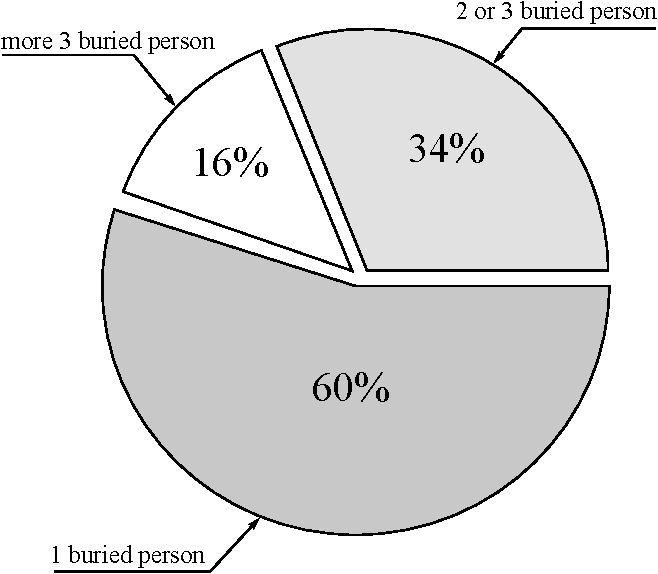
\includegraphics[width=5cm]{ch1/img/statistiche_sepolti.pdf}
	\caption{Number of buried}
\end{marginfigure}

Another important factor is the position of the overwhelms hikers:
\begin{itemize}
\item 37\% remain on the surface of the avalanche
\item 28\% are only partially buried
\item 35\% are completely buried
\end{itemize}

The survival curve, because of frostbite and hypothermia, without considerable traumas, has an upper limit of 15--18 minutes. Here is the the companion rescue that makes the real difference\cite{ManualeSciAlpinismo}.

One last important statistic is the number of hikers found with the ARTVA\marginnote{ARTVA: from the Italian \emph{Apparecchio Ricerca Travolti VAlanga}}. Considering the fact that the statistics do not take into account the episode of auto-rescue, the 7\% of the buried are found by the use of the receivers, a very small amount of the total. This data should be revised in the light of the advent of new digital ARTVA receivers, that simplify the searching method, and reduce the searching time \citep{hereforddigital}. 

As reported in \citep{Brugger2007}, within Europe and North America, avalanche airbags and avalanche transceiver reduce mortality, and companion rescue reduces incredibly the median duration of burial, remarking the extreme importance of those device for all mountaineers.

It is also known that 95\% of complete burial are in the layer between \num{-3} and\num{0} \si{\meter} of the avalanche.

\section{Avalanche Beacons}

There are two main typologies of avalanche transceiver. Differences are mostly in the user interface during receiving. We can divide in \emph{analog} and \emph{digital} ARTVA. Both device are equal for what concerns transmission. ARTVA can not be at the same time in transmission mode and receiving mode. Some models switch from receiving to transmission status after a scheduled amount of time. 

\subsection{Transmission Mode}

During transmission, beacons transmit a so-called \emph{wild-life tag}, or more simply, an intermittent signal at defined frequency, as stated in normative\cite{NormativaARVA}. From the normative, it is possible to extract more informations about the transmitted signal, that are listed in section \ref{sec:a1asegnale}.

\subsection{Receiving Mode}

The normative states for receiver:
\begin{itemize}
	\item the $(S+N)/N$ ratio of \num{6}\si{\decibel} at the terminal of electro--acoustic transducer
	\item a clear optical indication of direction for beacon with optical signal indication of direction
\end{itemize}
\marginnote{The Italian authority in Mountain Rescue is \emph{Soccorso Alpino e Speleologico Italiano}}

\myparagraph{Analog Beacons}
The analog beacon uses a cascade of filters and an identification circuit to extract the strength information of received signal. The strength is thus used as gain command for a sound generator, that rescuer uses to identify the direction of arrival. Typically, those ARTVA have a volume knob to perform a fine search. The main drawback is the extreme difficulty to perform a fast search, that requires an experienced user. Quoting \citep{457andfuture}: \emph{a better term for analog beacon would be \textbf{audible--based}}

\myparagraph{Digital Beacons}
Those beacons implements an user interface that indicates \emph{the field line direction and an artificial distance to the center of the field}. This simplicity makes those beacons perfect for unexperienced user and auto-rescue: those device \textbf{are strongly advised by the Mountain Rescue for all hikers, experienced or not}.

\begin{marginfigure}
	\centering
	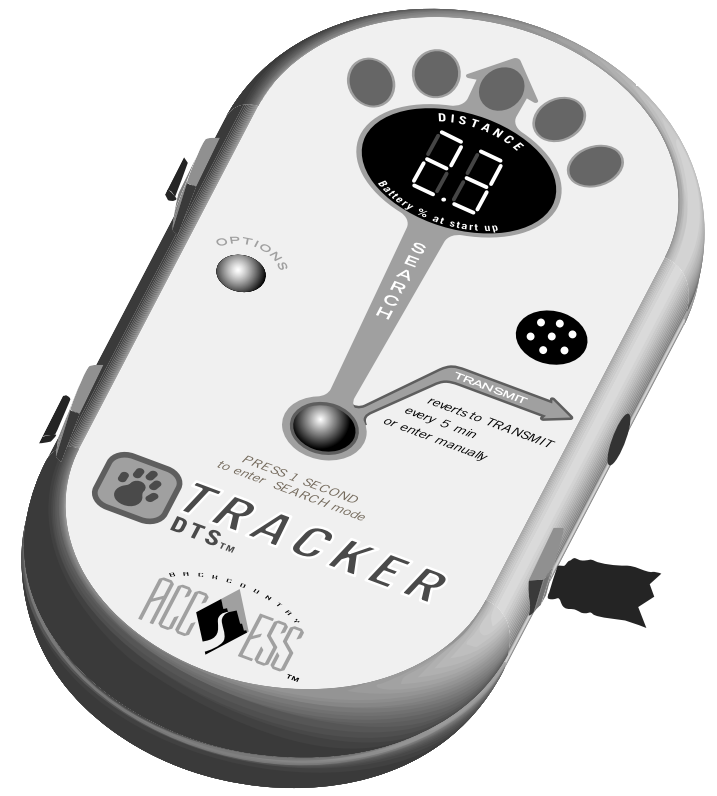
\includegraphics[width=4cm]{ch1/img/digital_baecon}
	\caption{Tracker DTS Avalanche Transceiver, a digital beacon}
\end{marginfigure}

Must be noted that the algorithm inside those transceivers runs on a very low power DPS, due to energy harvesting requirements, so often the rescuer must slow down his speed to gave time to the beacon to analyze received data. Also, it was pointed out from manufacturers that advanced techniques, like multi-buried identification and buried status (hearth-beat) make use of frequencies different from the one described in normative.

\subsection{Italian Mountain Rescue Intervention}
What happens after an avalanche? We interviewed some of the professionals of the Mountain Rescue Team in province of Trento, and asked them to explain us the actual procedure.

\myparagraph{Intervention on Avalanche}
The intervention begin after a witness call. Usually the witness is one of the hikers that is on the accident location. In the best situation, the witness begins the companion rescue procedure, with his own avalanche beacon, and calls the emergency number.

During the emergency call, the operator tries to understand the location, alerts the rescue team on shift and tries to figure out the general situation that the team may encounter. A rescue unit is formed by:
\begin{itemize}
\item Mountain Rescue heli-ambulance expert
\item Mountain Rescue canine unit
\item Health equip and nurse
\end{itemize}
If heli-ambulance is cleared to take off, those are the first rescuers on the avalanche. The clearance is related to weather and light conditions, because flight is performed by eye-sight. If heli-ambulance mission is aborted, Mountain Rescue team have to reach the avalanche with ground vehicle.

Under certain strict condition, it is possible to perform an ARTVA search from the helicopter.

Once arrived on the location, if residual risk make it possible, the rescue team is dropped from the heli-ambulance and starts the searching procedure, with canine unit and with personal ARTVAs. The rescuers with the beacons follow a scheme that allow them to cover the avalanche front. This scheme is called primary search. While a signal is identified, the rescuer start a fine search to pinpoint the buried position.

\myparagraph{Equipment}
There is a procedural and moral obligation in having the last generation device, even if does not exist a directive that defines a specific model for the equipment. Each rescuer has a VHF transmitter and cellphone, along with the personal beacon. 

It is possible to perform a search with other technology, like RECCO\sidenote[]{RECCO is a passive searching method, composed by a reflector included in hikers clothing, and a detector used by rescue teams. A RECCO detector usually performs passive search and \num{457}\si{\kilo\hertz} avalanche beacons search at the same time. The last generation detector has an average weight of \num{1}\si{\kilogram}, while the reflector weights only few grams. RECCO cannot be used for companion rescue}, even if the detector is heavy and not always reliable.

\section{State of the Art}

In this section we will analyze the state of the art in the field of beacons construction and signal analysis.

\subsection{Transmission}

Normative states the use of a very long wavelength ($\lunghezzaonda$) (\num{656}\si{\meter}). Such a long wavelength reduces the interference effects of snow, body and rocks and also multi-bouncing and multi-path effects\citep{balanis2012antenna} that may afflict some shorter waves. This is one of the main reason why GPS technology never erupted in this field\citep{457andfuture}.

This advantage also bring a consistent number of drawbacks, such as the fact that the search is always performed in near--field (distance less of $\lunghezzaonda/2\pi$). In the near--field, as we will see, interpretation of flux lines is quite complex, and it is difficult to derive a general direction of arrival algorithm.

Avalanche transceiver for companion rescue has to be small, therefore antennas and batteries has to be small. As we will see in the next chapter, to increase receiver antenna gain (also called effective height $\altezzaeffettiva$), ferrite core antennas are commonly used, but the efficiency and the noise introduced is not good. Those brings to transmitter that may be identified in the range of \numrange{40}{60}\si{\meter}, in function of type of receiver.

There is no big evolution in transmitters; almost all devices implement a simple amplitude--shifting--key (ASK) transmitter, build with an oscillator for the carrier, and a variable gain amplifier that modulates the intelligence signal.

\subsection{Reception}

Usually, an analog receiver has a little more bigger receiving radius with respect to a digital one. This difference is due to stronger filtration routines implemented in digital ARTVA, with respect to analog, and because of the dimension of the z--axis antenna.

A digital ARTVA implements multiple antennas. Some typical configurations are:
\begin{itemize}
\item two crossing antennas
\item three perpendicular antennas
\end{itemize}
The signal from whips are preprocessed using analog circuitry and then converted and processed in a DSP microprocessor. There are some advanced techniques\citep{Salos2007} implemented for the identification of the direction of the vectorial H--field, and also to help hikers and rescuers to find a transmitter. 

In general, the circuit may be resumed as follows:

\begin{figure}
	\centering
	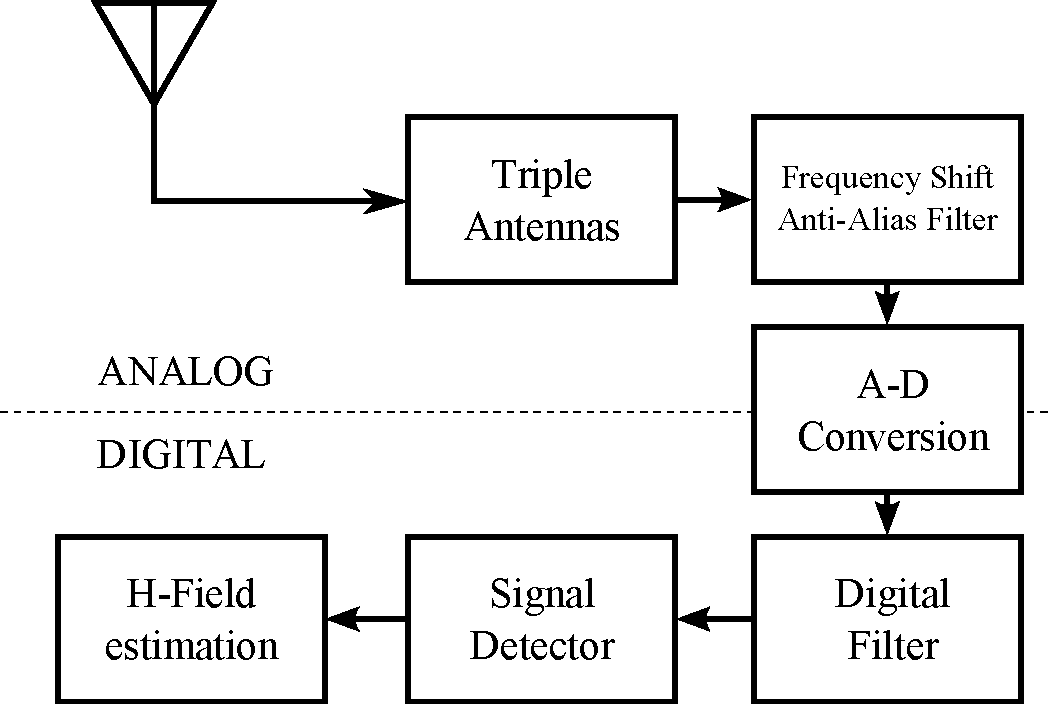
\includegraphics[width=7cm]{ch1/img/img_schema_arva.pdf}
	\caption{Block diagram of a commercial digital beacon, taken from \citep{Salos2007}}
	%\forceversofloat
\end{figure}


\begin{itemize}
\item signal is received through the antennas
\item the first stage of filtering is a frequency shift and  an anti-aliasing filter, that is necessary to avoid problems during AD-conversion
\item the signal is converted in the digital domain
\item other filtration techniques are analyzed  in \citep{Salos2007}, and are one of the main research topic in this field, in association with phase analysis to better understand the direction of the single components of the H--field
\item the signal detector and magnetic field estimator is implemented via software
\end{itemize}

One of the main challenge is the problem of the noise introduced by antennas. This noise is proportional to the received signal, phenomenon that induces an unsurmountable issue in the identification of multiple burial signal.

\subsection{Searching Algorithms}

\myparagraph{The magnetic momentum problem}
The main problem is the searching of the burial. Until now, only few are the example of automatic searching, while quite consolidated is the practice of the manual searching. One of the key aspects is the problem of the orientation of the transmitter: as we will see in the next chapter, the direction of the transmitter antenna change radically the shape of the field. From a general point of view, with respect to classical far--field identification problem, in this case we have to identify 6 state for each transmitter\sidenote[]{3 states refer to the position of the transmitter, while the latter 3 refers to the magnetic dipole momentum that is parallel to the axis of the antenna}, instead of 3, while we can only collect 3 measurements (the H--field vector components).

Even if there are some solutions for near--field qualitative direction of arrival, as explained in detail in \citep{hutchinson2000arrl}, typically those algorithms require a very prohibitive electro--mechanical circuitry, not suitable as mountain equipment (or in our case, a drone).

So far, only one solution earns the right to be cited: the solution proposed in \citep{pinies2006fast,pinies2006localization}, based upon Bayesian estimation theory and Kalman filters, is a remarkable attempt to find new approach to this problem, even if based on the weak assumption of a perfect knowledge of the covariance matrix related to the noise. One step ahead in this direction should be the redefinition of the problem in a dual form, from the Kalman filter to the information filter, in which the complete uncertainty is presented with a null matrix of the canonical form, instead of a infinite--valued matrix of the normal form. 

\myparagraph{Multiple Burial}
Those algorithms do not analyze the problem of multiple burial, and the subsequent possible situation of overlapping signal. An almost complete dissertation about this problem, with some test on beacon present on the market, may be found in \citep{signaloverlappingARVA1,signaloverlappingARVA2}. From those technical documents, distributed by one of the most well-know company in snow--safety, rises the evident lack of a solution for the overlapping problem, due to transmitted signal limitation. The most suggest solution is to run--away from an identified source in the hope to find another new signal. Some producer try to avoid this using parallel carrier frequency with additional information coded into intelligence signal (unique ID, heartbeat status, \dots). Those alternative frequencies are device/model dependent.

\myparagraph{A complex procedure}
Standard de facto is an algorithm of flux line following, in parallel with different assumption that user shall analyze, to derive the possible orientation of the buried person transmitting antenna, and subsequently find the best way to reach the hikers position. The complete explanation for the searching procedure is long even if not too complex, but based upon qualitative observation and deduction derived from expertise of the rescuer.

Generally speaking, what we need to know is the fact that a simple translation of this procedure in a machine with limited computational power is not practically possible.

A comprehensive description of the companion search and Mountain Rescue procedure could be found in \citep{ManualeSciAlpinismo}.

\section{Autonomous VTOL for buried searching}

The thesis is built around the main thread of inspect and derive the avionics of an autonomous VTOL. Even if avionics refer to the complete set of instrumentation and algorithms necessary to stabilize and control the flight, in this work we will focus on some of the main aspects necessary to perform the main task of buried searching.

This work is not the first attempt to bring an automatic drone on avalanches. Some remarkable examples are 
\begin{itemize}
\item SHERPA, European project born to create a robotic framework of helpers for Mountain Rescue, coordinated by University of Bologna
\item An user--piloted quad-copter research is just started in Politecnico di Torino
\item the project Alcedo from the Eidgen\"{o}ssische Technische Hochschule Z\"{u}rich\cite{projectAlcedoZurigo}
\end{itemize}

\subsection{Why the use of a VTOL?}
The use of a drone in the searching area depends on various factors. During design it is necessary to understand and think a system the fit entirely the actual search strategy.

One practical example of use could be a situation of high residual danger and an uncertainty about the presence of buried under the avalanche. In a case like that, the VTOL could be used to test the necessity of drop the rescue team on the avalanche.

The main advantage is obviously the ability to move faster on the avalanche with respect to an human rescuer, avoiding ground difficulties. At the same time, the drone should be able to identify and avoid obstacle like trees and ski--lift pillars.

\subsection{Quality Function Deployment}
The best way to define the characteristics of a new product is to inspect customer needs, and from qualitative user domain extrapolate quantitative engineering dimensions\cite{akao1994development}.

\myparagraph{Customer Needs}
From our interviews of Mountain Rescue members, we have derived some conclusions:
\begin{itemize}
\item one of the main cause of an avalanche is the weather, that modifies snow characteristics; during one day multiple avalanches may fall, so it is fundamental to guarantee a long, even if discontinue, operative time
\item the VTOL should be portable, with limited size and weight, but at the same time ready to be used in a short amount of time
\item all design process should take in to account the extreme low temperature and the high altitude (lower air density)
\item ARTVA device on the drone has to be robust with respect to electromagnetic interferences (propeller engines, radio, \dots)
\item user interface is simple while complete
\item the marking of the victims shall be hardware, with the use of visible darts
\end{itemize}
\begin{margintable}
	\begin{center}
		\begin{tabular}{ p{3.7cm} p{0.7cm} }
			\hline \textbf{Customer Need} & \textbf{Rating} \\ \hline
			Identifies buried person & 5 \\
			Is autonomous & 5 \\
			Returns to rescuer position & 5 \\
			Searches for the signall & 5 \\
			Is fast & 5 \\
			Marks physically buried position & 5 \\
			Operates at avalanche temperatures & 5 \\
			Performs more than one operation during the day & 3 \\
			Is usable by anyone & 3 \\
			Is robust with respect to EM interferences & 5 \\
			Is portable in a \num{35}\si{\liter} bag & 3 \\
			Is quiet & 2 \\
			Is compatible with other rescue vehicles & 5 \\
			Disengages from the winch & 5 \\
			Respects ENAC normatives & 3 \\
			\hline
		\end{tabular}
	\end{center}
	\caption{Customer needs \label{tbl:customer_needs}}
\end{margintable}

We are now able to define a table \ref{tbl:customer_needs} in which at each customer needs a rating is given.

In future, the automatic recognition of the avalanche dimensions could be a good starting point for some advanced research in the field of computer vision, or the improvements of user interface using voice recognition over radio.

\myparagraph{Technical Specification}
The next step in the definition of a good design is a list of technical specifications that will help us to identify the most challenging problems in and the gravity of those problems with respect to the costumer needs.

For sure, one of the first and most challenging complication is the weight reduction, that guarantees a longer flying time. Also those elements are related to the number of  propulsion vector and the main dimension (the length of the arm). It is evident the correlation between the number of lift vectors with respect to the maximum wind interference.

For the definition of a good searching algorithm, as we will see, it is important a good resolution of position and attitude of the drone; while to avoid obstacle it is important the resolution and the maximum revealing distance of the range finders.

One final aspect that should be considered are the data related to the system that performs the marking of a buried person.

All the specifications are listed in table \ref{tbl:tech_specs}
\begin{margintable}
	\begin{center}
		\begin{tabular}{ p{3.7cm}  p{0.7cm} }
			\hline \textbf{Technical Spec.} & \textbf{Dim.}  \\ \hline
			Flying time & \si{\minute} \\
			Weight & \si{\kilogram} \\
			N. of antennas & ~ \\
			Battery Temperature & \si{\celsius} \\
			Range Ultrasonic RF & \si{\meter} \\
			Arm Length & \si{\meter} \\
			Control TX distance & \si{\meter} \\
			GPS Resolution & \si{\meter} \\
			Lateral Speed & \si{\meter\per\second} \\
			 Wind Speed & \si{\meter\per\second} \\
			 ARTVA RX distance & \si{\meter} \\
			 Resolution Ultrasonic RF & \si{\meter} \\
			 Lift Force & \si{\newton} \\
			 N. dissembled pieces & ~ \\
			 N. Darts & ~ \\
			 N. Lift Vector & ~ \\
			 Maximum inclination & \si{\radian} \\
			 Operative height & \si{\meter} \\
			 IMU Resolution & \si{\meter\per\second} \\
			 Weight Marking Device & \si{\kilogram} \\
			 Weight Dart & \si{\kilogram} \\
			 Weight ARTVA & \si{\kilogram} \\
			\hline
		\end{tabular}
	\end{center}
	\caption{Technical specifications \label{tbl:tech_specs}}
\end{margintable}

% TODO invertire colonna 1 e 2 e nella nuoova colonna 2 inserire la dimensione 

\myparagraph{Merging the tables and comparison}
In table \ref{tbl:need_vs_spec} all data are compared with a weighting method. The table shows the comparison between technical specifications and customer needs and also between technical specifications and the other technical specifications.

\myparagraph{Components selection}
From the merged data it was possible to select the components that will be used in the prototype. All components are listed in table \ref{tbl:components_list}

We have also decide not to use a commercial ARTVA, but instead try to build a digital one from scratch. This will allow us to get a lighter model, and also extract exactly the information that we want from the received signal. Even if some device have a serial port, the output data are filtered with models that incorporate the possible speed of a rescue, that is different from our VTOL.
\begin{table}
	\begin{center}
		\begin{tabular}{ p{0.3cm} p{3.7cm} p{3.7cm} p{1cm} }
			\hline \scriptsize{\textbf{N}} & \footnotesize{\textbf{Component}} & \scriptsize{\textbf{Description}} & \footnotesize{\textbf{Price}} \\ \hline
			\scriptsize{$1\times$} & \footnotesize{Autoquad 6 Flight Controller} & \scriptsize{Imu board and stabilization controller} & \footnotesize{299.00\texteuro} \\
			\scriptsize{$6\times$} & \footnotesize{Autoquad ESC32} & \scriptsize{Electronic speed controller} & \footnotesize{239.40\texteuro} \\
			\scriptsize{$6\times$} & \footnotesize{Flyfuino HE4108 700kV Outrunner} & \scriptsize{Motors} & \footnotesize{299.40\texteuro} \\
			\scriptsize{$6\times$} & \footnotesize{HQ 12\inch per 4.5\inch CW and CCW Carbon propeller} & \scriptsize{Propeller} & \footnotesize{73.80\texteuro} \\
			\scriptsize{$2\times$} & \footnotesize{SLS Xtron \num{5000}\si{\milli\ampere\hour} \num{14.8}\si{\volt}} & \footnotesize{Batteries} & \footnotesize{119.98\texteuro} \\
			\scriptsize{$3\times$} & \footnotesize{USB UART Adapter} & \scriptsize{Bridge between USB and device UART} & \footnotesize{9.90\texteuro} \\
			\hline
			\multicolumn{3}{r}{\footnotesize{\textbf{Total}}}  & \footnotesize{1041.48\texteuro} \\
			\hline
		\end{tabular}
	\end{center}
	\caption{Components list \label{tbl:components_list}}
\end{table}

\newcommand{\rotatenovsmalll}[1]{\begin{sideways}\scriptsize{\textbf{#1}}\end{sideways}}
\newcommand{\smallbold}[1]{\scriptsize{\textbf{#1}}}

%\def\nine{\scriptsize{\textbf{9}}}
%\def\three{\scriptsize{3}}
\def\nine{\scriptsize{$\CIRCLE$}}
\def\three{\scriptsize{$\RIGHTcircle$}}
\def\point{\scriptsize{$\ocircle$}}

\def\upnin{\scriptsize{\begin{sideways}$\RHD$\end{sideways}}}
\def\upthr{\scriptsize{\begin{sideways}$\rhd$\end{sideways}}}
\def\dwnin{\scriptsize{\begin{sideways}$\LHD$\end{sideways}}}
\def\dwthr{\scriptsize{\begin{sideways}$\lhd$\end{sideways}}}

\begin{table*}[p]
    \centering
    \begin{tabular}{ b{4cm} b{0.08cm} b{0.08cm} b{0.08cm} b{0.08cm} b{0.08cm} b{0.08cm} b{0.08cm} b{0.08cm} b{0.08cm} b{0.08cm} b{0.08cm} b{0.08cm} b{0.08cm} b{0.08cm} b{0.08cm} b{0.08cm} b{0.08cm} b{0.08cm} b{0.08cm} b{0.08cm} b{0.08cm} b{0.08cm} }
    \hline
    \smallbold{Identifies buried person}                            &  \nine   &  \point  &  \nine   &  \point  &  \point  &  \point  &  \point  &  \nine   &  \three  &  \point  &  \nine   &  \point  &  \point  &  \point  &  \nine   &  \point  &  \point  &  \point  &  \point  &  \three  &  \three  &  \three  \\
    \smallbold{Is autonomous}                                       &  \three  &  \nine   &  \nine   &  \point  &  \nine   &  \point  &  \nine   &  \nine   &  \three  &  \nine   &  \nine   &  \three  &  \point  &  \point  &  \point  &  \point  &  \point  &  \point  &  \nine   &  \point  &  \point  &  \point  \\
    \smallbold{Returns to rescuers position}                        &  \nine   &  \point  &  \point  &  \point  &  \point  &  \point  &  \nine   &  \nine   &  \three  &  \nine   &  \point  &  \nine   &  \point  &  \point  &  \point  &  \point  &  \point  &  \three  &  \three  &  \point  &  \point  &  \point  \\
    \smallbold{Searches for the signal}                             &  \nine   &  \point  &  \nine   &  \point  &  \point  &  \point  &  \point  &  \nine   &  \nine   &  \point  &  \nine   &  \point  &  \point  &  \point  &  \point  &  \point  &  \point  &  \nine   &  \three  &  \point  &  \point  &  \nine   \\
    \smallbold{Is fast}                                             &  \three  &  \nine   &  \point  &  \point  &  \three  &  \nine   &  \point  &  \nine   &  \point  &  \nine   &  \point  &  \nine   &  \nine   &  \point  &  \point  &  \nine   &  \nine   &  \point  &  \nine   &  \three  &  \point  &  \point  \\
    \smallbold{Marks physically buried position}                    &  \point  &  \point  &  \point  &  \point  &  \point  &  \point  &  \nine   &  \nine   &  \point  &  \nine   &  \point  &  \nine   &  \point  &  \point  &  \nine   &  \point  &  \point  &  \point  &  \nine   &  \three  &  \nine   &  \point  \\
    \smallbold{Operates at avalanche temperature}                   &  \point  &  \point  &  \point  &  \nine   &  \point  &  \point  &  \nine   &  \nine   &  \point  &  \nine   &  \point  &  \nine   &  \point  &  \point  &  \point  &  \point  &  \point  &  \nine   &  \nine   &  \nine   &  \point  &  \point  \\
    \smallbold{Performs more than one operation during the day}     &  \nine   &  \three  &  \point  &  \nine   &  \point  &  \point  &  \point  &  \point  &  \point  &  \point  &  \point  &  \point  &  \three  &  \point  &  \three  &  \three  &  \point  &  \three  &  \point  &  \point  &  \three  &  \point  \\
    \smallbold{Is usable by anyone}                                 &  \point  &  \point  &  \point  &  \point  &  \three  &  \point  &  \three  &  \point  &  \point  &  \point  &  \point  &  \point  &  \point  &  \nine   &  \point  &  \point  &  \point  &  \point  &  \point  &  \three  &  \point  &  \point  \\
    \smallbold{Is robust with respect to EM}                        &  \point  &  \point  &  \nine   &  \point  &  \point  &  \point  &  \nine   &  \nine   &  \point  &  \nine   &  \three  &  \point  &  \point  &  \point  &  \point  &  \nine   &  \point  &  \point  &  \nine   &  \point  &  \point  &  \nine   \\
    \smallbold{Is portable  in a 35L bag}                           &  \point  &  \nine   &  \point  &  \three  &  \point  &  \nine   &  \point  &  \point  &  \point  &  \point  &  \point  &  \point  &  \point  &  \nine   &  \nine   &  \nine   &  \point  &  \point  &  \point  &  \point  &  \three  &  \nine   \\
    \smallbold{Is quiet}                                            &  \point  &  \point  &  \point  &  \point  &  \point  &  \point  &  \point  &  \point  &  \three  &  \point  &  \point  &  \point  &  \three  &  \point  &  \point  &  \nine   &  \three  &  \point  &  \point  &  \nine   &  \point  &  \point  \\
    \smallbold{Is compatible with other rescue vehicles}            &  \point  &  \point  &  \nine   &  \nine   &  \point  &  \point  &  \point  &  \nine   &  \point  &  \point  &  \nine   &  \point  &  \point  &  \point  &  \point  &  \point  &  \point  &  \point  &  \point  &  \point  &  \point  &  \point  \\
    \smallbold{Disengages from the winch}                           &  \point  &  \three  &  \point  &  \three  &  \point  &  \three  &  \point  &  \point  &  \point  &  \point  &  \point  &  \point  &  \point  &  \point  &  \point  &  \point  &  \point  &  \point  &  \point  &  \point  &  \nine   &  \nine   \\
    \smallbold{Respects ENAC normatives}                            &  \point  &  \nine   &  \three  &  \nine   &  \nine   &  \nine   &  \nine   &  \three  &  \three  &  \three  &  \point  &  \nine   &  \point  &  \point  &  \point  &  \nine   &  \point  &  \nine   &  \point  &  \three  &  \three  &  \three  \\
    \hline \\ 


    \scriptsize{\textbf{Legend}: \newline \scriptsize{\emph{Cust. needs vs. Tech. spec.}: \newline\point \hspace{1.5mm} no relation \newline\three \hspace{1.5mm} light relation \newline\nine \hspace{1.5mm} strong relation \newline \emph{Tech. spec. vs. Tech. spec.}: \newline\dwnin \hspace{1.5mm} negative strong relation \newline\dwthr \hspace{1.5mm} negative light relation \newline\point \hspace{1.5mm} no relation \newline\upthr \hspace{1.5mm} positive light relation \newline\upnin \hspace{1.5mm} positive strong relation}}

     & \rotatenovsmalll{Flying time} & \rotatenovsmalll{Weight} & \rotatenovsmalll{N. ARTVA antennas} & \rotatenovsmalll{Battery Temperature} & \rotatenovsmalll{Range Ultrasonic RF} & \rotatenovsmalll{Arm Length} & \rotatenovsmalll{Control TX distance} & \rotatenovsmalll{GPS resolution} & \rotatenovsmalll{Lateral speed} & \rotatenovsmalll{Wind speed} & \rotatenovsmalll{ARTVA RX distance} & \rotatenovsmalll{Resolution Ultrasonic RF} & \rotatenovsmalll{Lift Force} & \rotatenovsmalll{N. dissembled pieces} & \rotatenovsmalll{N. Darts} & \rotatenovsmalll{N. Lift vector} & \rotatenovsmalll{Maximum inclination} & \rotatenovsmalll{Operative Height} & \rotatenovsmalll{IMU resolution} & \rotatenovsmalll{Weight Marking Device} & \rotatenovsmalll{Weight Darts} & \rotatenovsmalll{Weight ARTVA}  \\
    \hline
    \multicolumn{2}{r}{\smallbold{Flying Time}}                                &  \dwnin  &  \dwthr  &  \dwthr  &  \point  &  \dwnin  &  \upthr  &  \upthr  &  \dwthr  &  \dwthr  &  \point  &  \point  &  \dwthr  &  \dwthr  &  \dwthr  &  \point  &  \point  &  \dwthr  &  \point  &  \dwnin  &  \dwnin  &  \dwnin  \\
    \multicolumn{3}{r}{\smallbold{Weight}}                                                &  \upnin  &  \upthr  &  \point  &  \upthr  &  \point  &  \point  &  \point  &  \upthr  &  \point  &  \point  &  \upthr  &  \upnin  &  \upnin  &  \upnin  &  \point  &  \point  &  \point  &  \upnin  &  \upnin  &  \upnin  \\
    \multicolumn{4}{r}{\smallbold{N. ARTVA antennas}}                                                &  \point  &  \point  &  \point  &  \point  &  \point  &  \point  &  \point  &  \upnin  &  \point  &  \dwthr  &  \upnin  &  \point  &  \point  &  \point  &  \point  &  \point  &  \point  &  \point  &  \upnin  \\
    \multicolumn{5}{r}{\smallbold{Battery temperature}}                                                         &  \point  &  \point  &  \point  &  \point  &  \dwthr  &  \point  &  \point  &  \point  &  \dwnin  &  \point  &  \point  &  \point  &  \point  &  \upnin  &  \point  &  \point  &  \point  &  \point  \\
    \multicolumn{6}{r}{\smallbold{Range Ultrasonic RF}}                                                                    &  \point  &  \point  &  \point  &  \upthr  &  \upthr  &  \point  &  \dwnin  &  \point  &  \point  &  \point  &  \point  &  \upnin  &  \point  &  \point  &  \point  &  \point  &  \point  \\
    \multicolumn{7}{r}{\smallbold{Arm length}}                                                                                        &  \point  &  \point  &  \upnin  &  \upnin  &  \point  &  \point  &  \dwthr  &  \point  &  \point  &  \point  &  \upthr  &  \point  &  \point  &  \point  &  \point  &  \point  \\
    \multicolumn{8}{r}{\smallbold{Control TX distance}}                                                                                          &  \upthr  &  \upthr  &  \point  &  \point  &  \point  &  \point  &  \point  &  \point  &  \point  &  \point  &  \point  &  \point  &  \point  &  \point  &  \point  \\
    \multicolumn{9}{r}{\smallbold{GPS Resolution}}                                                                                                          &  \point  &  \upthr  &  \point  &  \point  &  \point  &  \point  &  \point  &  \point  &  \point  &  \point  &  \dwthr  &  \point  &  \point  &  \point  \\
    \multicolumn{10}{r}{\smallbold{Lateral speed}}                                                                                                                     &  \point  &  \point  &  \point  &  \upnin  &  \point  &  \point  &  \upnin  &  \upnin  &  \point  &  \point  &  \point  &  \point  &  \point  \\
    \multicolumn{11}{r}{\smallbold{Wind speed}}                                                                                                                                   &  \point  &  \point  &  \upnin  &  \point  &  \point  &  \upnin  &  \upthr  &  \point  &  \upnin  &  \upthr  &  \upthr  &  \upthr  \\
    \multicolumn{12}{r}{\smallbold{ARTVA RX distance}}                                                                                                                                       &  \point  &  \point  &  \point  &  \point  &  \point  &  \point  &  \point  &  \point  &  \point  &  \point  &  \upnin  \\
    \multicolumn{13}{r}{\smallbold{Resolution Ultrasonic RF}}                                                                                                                                           &  \point  &  \point  &  \point  &  \point  &  \point  &  \point  &  \point  &  \point  &  \point  &  \point  \\
    \multicolumn{14}{r}{\smallbold{Lift Force}}                                                                                                                                                                    &  \point  &  \point  &  \upnin  &  \upthr  &  \upnin  &  \point  &  \point  &  \point  &  \point  \\
    \multicolumn{15}{r}{\smallbold{N. disassembled pieces}}                                                                                                                                                                   &  \upnin  &  \upnin  &  \point  &  \point  &  \point  &  \upthr  &  \upthr  &  \upthr  \\
    \multicolumn{16}{r}{\smallbold{N. Darts}}                                                                                                                                                                                            &  \point  &  \point  &  \point  &  \point  &  \upnin  &  \dwnin  &  \point  \\
    \multicolumn{17}{r}{\smallbold{N. Lift vector}}                                                                                                                                                                                                 &  \upnin  &  \upnin  &  \point  &  \point  &  \point  &  \point  \\
    \multicolumn{18}{r}{\smallbold{Maximum inclination}}                                                                                                                                                                                                       &  \dwthr  &  \point  &  \point  &  \point  &  \point  \\
    \multicolumn{19}{r}{\smallbold{Operative Height}}                                                                                                                                                                                                                     &  \point  &  \point  &  \point  &  \point  \\
    \multicolumn{20}{r}{\smallbold{IMU Resolution}}                                                                                                                                                                                                                                  &  \point  &  \point  &  \point  \\
    \multicolumn{21}{r}{\smallbold{Weight Marking Device}}                                                                                                                                                                                                                                      &  \upnin  &  \point  \\
    \multicolumn{22}{r}{\smallbold{Weight Darts}}                                                                                                                                                                                                                                                          &  \point  \\
    \end{tabular}
    \caption{Comparison Table\label{tbl:need_vs_spec}}
    \forceversofloat
\end{table*}

%\marginnote{\textbf{How to read table \ref{tbl:need_vs_spec}}: \newline \scriptsize{\emph{Cust. needs vs. Tech. spec.}: \newline\point \hspace{1.5mm} no relation \newline\three \hspace{1.5mm} light relation \newline\nine \hspace{1.5mm} strong relation \newline \emph{Tech. spec. vs. Tech. spec.}: \newline\dwnin \hspace{1.5mm} negative strong relation \newline\dwthr \hspace{1.5mm} negative light relation \newline\point \hspace{1.5mm} no relation \newline\upthr \hspace{1.5mm} positive light relation \newline\upnin \hspace{1.5mm} positive strong relation}}

\let\nine\undefined
\let\three\undefined
\let\point\undefined
\let\upnin\undefined
\let\upthr\undefined
\let\dwthr\undefined
\let\dwnin\undefined

\FloatBarrier

	% CHAPTER 2

\chapter{Design of a digital ARTVA \label{ch:chapter2}}
\minitoc
%% Enlarge array size
\renewcommand{\arraystretch}{2}

In this chapter we will try to design a digital receiver for the ARTVA signal. Before starting with the design, \emph{ARTVA signal} is deeply analyzed, with the derivation of a simplified model for a field pattern that could be used  for the implementation of the searching algorithm. After that, ferrite antennas are studied, as they are the only way to receive such a long wavelength. In the last part of the chapter the circuitry for the ARTVA receiver is shown and explained.

\section{Analysis of transmitting pattern}

A formal model of the transmitting pattern is fundamental for the implementation of the searching algorithm. We start from the basic Maxwell's equation and we arrive to a simpler model numerically usable.

As we will see, radiating pattern is quite complex due to the fact that we are working in the \textbf{near--field} region, condition that constraint us to not use classical DoA\marginnote{\emph{DoA}: Direction of Arrival}, such as MUSIC or ESPRIT, that operates in far-field condition and at higher frequencies. DoA systems for long waves usually requires too big electro--mechanical devices.

\subsection{Maxwell's Equations}
The following investigation is based upon Maxwell's Equation, in which the magnetic permeability $\magperm$ and dielectric constant $\dielettrico$ are considered constant (the radiation is assumed to propagate at speed of light in air). Also we consider some field properties, that are function of radio distance $\radiodist$ and time $t$:
\[
f(\radiodist,t) = f \qquad f \in \left[\; \chargedens,\; \currdens,\; \efield,\; \bfield,\; \hfield \; \right]
\]
The equations that rule the induction are the \emph{Gauss equation of magnetic induction} and the \emph{Faraday law of electric induction}:
\begin{equation}
\nabla\cdot\bfield = 0
\label{eq:gauss1}
\end{equation}
\begin{equation}
\nabla\times\efield = -\partialt \bfield
\label{eq:faraday}
\end{equation}
while the equations that rule the interaction with materials are \emph{Gauss equation} and \emph{Ampere law}:
\begin{equation}
\nabla\cdot\efield = \dfrac{\chargedens}{{\dielettrico}_0}
\label{eq:gauss2}
\end{equation}
\begin{equation}
\nabla\times\bfield = {\magperm}_0 \left( \currdens + {\dielettrico}_0 \partialt \efield \right)
\label{eq:ampere}
\end{equation}

\subsection{EM field dynamic potentials}

Starting from equation \ref{eq:gauss1}, we can define a vectorial function called \emph{potential vector} $\afield$ of $\bfield$:
\begin{equation}
\bfield = \nabla\times\afield
\label{eq:potvett}
\end{equation}
\marginnote{The existence of $\afield$ is verified by property of $\nabla$ operator, whom states that the divergence of a curl of a vector field is zero\citep{bramanti2009analisi}} 
We insert \ref{eq:potvett} in \ref{eq:faraday}:
\[
\nabla\times\efield = - \partialt \left( \nabla\times\afield \right)
\]
\begin{equation}
\nabla\times\left( \efield + \partialtarg{\afield} \right) = 0
\end{equation}
From the previous equation it is evident that the argument between parentheses is an irrotational vector field, thus a potential function exists such that:
\[
-\nabla\scpot = \efield + \partialtarg{\afield}
\]
and we derive the following definition of electric field:
\begin{equation}
\efield = - \nabla \scpot - \partialtarg{\afield}
\label{eq:efieldvett}
\end{equation}
Equation \ref{eq:potvett} and \ref{eq:efieldvett} are used to express a new formulation for the Maxwell's equation based upon vector potential\sidenote{The proof is in chapter appendix \ref{eq:evidence1}}:
\begin{equation}
\begin{array}{rcl}
\nabla^2\scpot + \partialt \nabla \cdot \afield & = & - \dfrac{\chargedens}{\dielettrico_0} \\
\nabla^2 \afield - \dfrac{1}{\velocitaluce^2} \partialttarg{\afield} - \nabla\left( \nabla \cdot \afield + \dfrac{1}{\velocitaluce^2} \partialtarg{\scpot} \right) & = & -\magperm_0 \currdens
\end{array}
\label{eq:potvecmaxwell}
\end{equation}
Those equation, even if complex, could be resolved with a well posed boundaries condition problem. Equation are coupled with the current formulation, but could be decoupled using the \textbf{Gauge transformation}\citep{mencuccini1988fisica}, also called \textbf{recalibration map}, that is in the form:
\begin{equation}
\left\{ \begin{array}{rcl}
\afield' & \mapsto & \afield + \nabla \lorentz \\
\scpot' & \mapsto & \scpot - \partialtarg{\lorentz}
\end{array}
\right.
\end{equation}
in which $\lorentz = \lorentz(\radiodist,t) \in C^2$. As proofed in \ref{eq:prooftransformationmap}, this map represents an invariant with respect to dynamic potential formulation. If we consider a $\lorentz$ such that it verifies the \textbf{Lorentz equation}
\begin{equation}
\nabla \cdot \afield' = - \dfrac{1}{\velocitaluce^2} \partialtarg{\scpot'}
\end{equation}
we obtain the decoupled version:
\begin{equation}
\begin{array}{rcl}
\nabla^2 \scpot - \dfrac{1}{\velocitaluce^2} \partialttarg{\scpot} & = & - \dfrac{\chargedens}{\dielettrico_0} \\
\nabla^2 \afield - \dfrac{1}{\velocitaluce^2} \partialttarg{\afield} & = & - \magperm_0 \currdens 
\end{array}
\end{equation}
Those dynamic equations describe the time evolution of an EM--field. If field sources are located in a finite region, the problem admit as solution a generalization of the well know stationary formulation, called retarded potential:
\begin{equation}
\begin{array}{rcl}
\scpot(\radiodist,t) & = & \dfrac{1}{4\pi \dielettrico_0} \displaystyle\iiint\limits_{\Omega} \dfrac{1}{\mid \radiodist - \radiodist' \mid} \chargedens\left( \radiodist',t-\dfrac{\mid \radiodist - \radiodist' \mid}{\velocitaluce} \right) d\radiodist   \\
\afield(\radiodist,t) & = & \dfrac{\magperm_0}{4\pi} \displaystyle\iiint\limits_{\Omega} \dfrac{1}{\mid \radiodist - \radiodist' \mid} \currdens\left( \radiodist',t-\dfrac{\mid \radiodist - \radiodist' \mid}{\velocitaluce} \right) d\radiodist 
\end{array}
\end{equation}
in which the vector distance ${\radiodist - \radiodist'}$ is the distance between the point where retarded potential is evaluated and the point where the element of volume $d\radiodist$ of the localized sources is located. The delay is due to the definition of time:
\[
t_r = t - \dfrac{\mid \radiodist - \radiodist' \mid}{c}
\]

\subsection{Magnetic dipole radiation}

\myparagraph{Potential of a magnetic dipole}
Our antenna may be seen as an ideal magnetic dipole\citep{balanis2012antenna}. The transmitting antenna is a solenoid with a ferrite core, that acts as source of the electro--magnetic field. The source is subject to a dipole magnetic moment induced by the current $J = J_0 \cos(\omegaarva t)$, with no free charges (null scalar potential). 
\begin{figure}[h]
	\centering
	
	\tdplotsetmaincoords{60}{130}
	\begin{tikzpicture}[auto,>=latex,tdplot_main_coords]
		\coordinate (origin) at (0,0,0);
		
		% Axis
		\draw [->] (origin) -- (4,0,0) node[anchor=north east]{\scriptsize{$x$}}; \draw (origin) -- (-0.2,0,0);
		\draw [->] (origin) -- (0,4,0) node[anchor=north west]{\scriptsize{$y$}}; \draw (origin) -- (0,-0.2,0);
		\draw [->] (origin) -- (0,0,2) node[anchor=south]{\scriptsize{$z$}}; \draw (origin) -- (0,0,-0.2);

		\tdplotdrawarc[->,line width=3]{(0,0,0)}{2.7}{90}{360+80}{}{}
		\tdplotdrawarc[line width=6]{(0,0,0)}{2.7}{25}{35}{}{}
		\tdplotdrawarc[<->]{(0,0,0)}{3.5}{0}{30}{anchor=north west,xshift=-10}{$\varphi'$}
		\coordinate (drpoint) at (30:2.7);
		\node at (-2.3,2.3,0) {$\mathbf{J}$};
		\node [at=(drpoint),xshift=5,yshift=-10] {$d\mathbf{r}$};

		\node [circle,draw,inner sep=1pt, fill=black] at (7.5,0,6) (rpoint) {};
		\draw[->] (origin) -- node[pos=0.8,above]{$\mathbf{r}$} (rpoint);
		\draw [dashed] (rpoint) -- (7.5,0,0) -- ++(-2.5,0,0);
		\coordinate [at=(drpoint),yshift=3] (drpoint2);
		\draw [<->] (rpoint) -- node[pos=0.425,below,xshift=-22]{$\kappa=|\mathbf{r}-\mathbf{r}'|$} (drpoint2);
		\draw [->] (origin) -- node[right]{$\mathbf{r}'$} (drpoint2);

		\tdplotsetrotatedcoords{90}{90}{180}
		\tdplotsetrotatedcoordsorigin{(origin)}
		\draw[tdplot_rotated_coords,<->] (0.5,0) arc (0:52.5:0.5) node[left,xshift=5,yshift=10]{$\theta$};

		\tdplotsetrotatedcoords{29.5+270}{-23.75}{0}
		\tdplotsetrotatedcoordsorigin{(origin)}
		\draw[tdplot_rotated_coords,<->] (0.75,0) arc (0:90:0.75) node[left,xshift=-15,yshift=10]{$\psi$};
		
	\end{tikzpicture}
	\tdplotsetmaincoords{0}{0}

	\caption{Formulation of magnetic dipole problem}
	\label{eq:dipolomagnetico}
	\forceversofloat
\end{figure}
The magnetic dipole moment is:
\begin{equation}
\magdipole = \pi r'^2\; J \vrz = m_0 \cos(\omegaarva t) \vrz
\label{eq:dipolodacorrente}
\end{equation}
From figure \ref{eq:dipolomagnetico} we define the retarded potential equation, with ${\kappa = \mid \radiodist-\radiodist'\mid}$:
\[
\afield(\radiodist,t) = \dfrac{\magperm_0}{4\pi}\int{\dfrac{J_0\cos(\omegaarva (t - \kappa/c))}{r}\ccos{\varphi'}d\varphi'}\hat{\boldsymbol{\phi}}
\]
In the hypothesis of ${\radiodist\parallel\vrz\times\vrx}$, we obtain a vector $\afield$ directed along $\vry$:
\[\begin{array}{rcl}
\radiodist & = & r \sin(\theta) \vrx + r \cos(\theta) \vrz \\
\radiodist' & = & r' \cos(\varphi') \vrx + r' \sin(\varphi') \vry \\
\kappa & = & \sqrt{(\radiodist - \radiodist')\cdot(\radiodist - \radiodist')}
\end{array}\]
Those elements in retarded potential formulation lead us to the integral formulation that has only one angular dependency:
\begin{equation}
\label{eq:integraledacalc}
\afield(\radiodist,t) = \dfrac{\magperm_0 J_0 r'}{4\pi}\int\limits_{0}^{2\pi}{\dfrac{\cos(\omegaarva (t - \kappa/c))}{\kappa} \cos(\varphi') d\varphi' \hat{\boldsymbol{\phi}}}
\end{equation}
The solution of this integral is reported in appendix; we recall only the simplification used:
\begin{itemize}
\item we assume $r' \ll r$
\item we assume $r' \ll \lambda = 2\pi c/\omegaarva$
\end{itemize}
that brings us to the following solution:
\begin{equation}
\label{eq:soluzioneint}
\afield(\radiodist,t) = \dfrac{\magperm_0 m_0}{4\pi r}\,\sin(\theta)\left( \dfrac{1}{r} \sin\left(\omegaarva(t-r/c)\right) - \dfrac{\omegaarva}{r}\cos\left(\omegaarva(t-r/c)\right)\right)\hat{\boldsymbol{\phi}}
\end{equation}
in which $m_0$ identifies the total dipole moment, considering also the number of the coils of antenna. The rest of the equation describes the propagation of the transmission in near--field conditions.

\myparagraph{Electric and magnetic field}
With null scalar potential we obtain the electric field and the magnetic field from the equations:
\begin{equation}
\begin{array}{rcl}
\efield & = & - \partialtarg{\afield} \\
\bfield & = & \nabla\times\afield 
\end{array}
\end{equation}
The application of differential operator $\nabla$:
\marginnote{In polar coordinates: \newline $\nabla=\left[ \begin{array}{c} \dfrac{\partial}{\partial r} \\ \dfrac{1}{r}\;\dfrac{\partial}{\partial\theta} \\ \dfrac{1}{r \sin(\theta)}\;\dfrac{\partial}{\partial\phi} \end{array} \right]$}
\begin{equation}
\efield = \left[ \begin{array}{c} 0 \\ 0 \\ \partialtarg{A_{\phi}} \end{array} \right]
\qquad
\bfield = \left[ \begin{array}{c} \dfrac{1}{r}\;\dfrac{\partial A_{\phi}}{\partial \theta} \\ - \dfrac{\partial A_{\phi}}{\partial r} \\ 0 \end{array} \right]
\end{equation}
The final formulation for th EM field of a magnetic dipole is\citep{knoepfel2008magnetic}:
\begin{equation}
\begin{array}{rcl}
\label{eq:campidef1}
\tau & = &  t - \dfrac{r}{\velocitaluce} \\
E_{\phi} & = & \dfrac{\magperm_0 m_0}{4\pi}\sin(\theta)\left( \dfrac{\omegaarva}{r^2}\sin\left( \omegaarva\tau \right) + \dfrac{\omegaarva^2}{c}\cos\left( \omegaarva\tau \right) \right) \\
B_{r} & = & \dfrac{\magperm_0 m_0}{2\pi r^2}\cos(\theta)\left( \dfrac{1}{r}\cos\left( \omegaarva\tau \right) + \dfrac{\omegaarva}{c}\sin\left( \omegaarva\tau \right) \right) \\
B_{\theta} & = & \dfrac{\magperm_0 m_0}{4 \pi r^3 c^2}\sin(\theta)\left( \left( \velocitaluce^2 - \omegaarva^2 r^2 \right)\cos\left( \omegaarva\tau \right) + \omegaarva r \velocitaluce \sin\left( \omegaarva\tau \right) \right) 
\end{array}
\end{equation}
In figure \ref{fig:animazionifield} are shown some animation referred to the magnetic field defined in the previous equations. The animation are performed using ARTVA typical parameters, even if time is scaled. The equations are parametric with respect to a value, $m_0$ that is the transmitter magnetic dipole. As we have seen in chapter \ref{ch:chapter1}, the real transmitting power of an avalanche beacon is not known, but it shall have the maximum at \num{10}\si{\meter} inside a range. The animations consider an unitary magnetic dipole moment.

\begin{figure*}[p]
\label{fig:animazionifield}
\animategraphics[width=6.5cm,autoplay,loop]{15}{ch2/img/xz_10m/animation_}{0}{59}
\animategraphics[width=6.5cm,autoplay,loop]{15}{ch2/img/xz_40m/animation_}{0}{59} \newline
\animategraphics[width=6.5cm,autoplay,loop]{15}{ch2/img/xz_100m/animation_}{0}{59}
\animategraphics[width=6.5cm,autoplay,loop]{15}{ch2/img/xz_2lambda/animation_}{0}{59} \newline
\animategraphics[width=6.5cm,autoplay,loop]{15}{ch2/img/xy_10m/animation_}{0}{59} 
\animategraphics[width=6.5cm,autoplay,loop]{15}{ch2/img/xy_2lambda/animation_}{0}{59}
\caption{Graphical animation of the magnetic field $\bfield$ with retarded potential formulation. Those graph derives directly from the equations \ref{eq:campidef1}. To see the animations, please use \texttt{Adobe Acrobat viewer}}
\end{figure*}

\subsection{Magnetic field model simplification}
From animations it is evident that the effect of retarded propagation is almost null inside a radius of \num{40}\si{\meter} from the transmitting source, that is roughly the maximum distance at which an avalanche beacon receives the signal. This brings us to other simplifications for our model, as we will see in this section. From now on, all the simplifications are performed with the intent to find a model computationally convenient to be used in our algorithms.

\myparagraph{Re--definition in complex domain}
The next step is to bring equation of magnetic field in complex domain, but keeping in mind that only real part of the equations retains the physical meaning of the field. The re--interpretation is based upon Euler relationship and on the definition of wavenumber:
\[
e^{j\beta} = \ccos{\beta} + j \ssin{\beta}
\]
\[
\numeroonda = \dfrac{\omegaarva}{\velocitaluce}
\]
\begin{equation}
\begin{array}{rcl}
B_r & = & \dfrac{1}{2} \dfrac{\magperm_0 m_0}{\pi} \ccos{\theta} \braces{\dfrac{1}{r^3}\ccos{\omegaarva \tau} - \dfrac{\kappa}{r^2} \ssin{\omegaarva \tau}} \\
 & = & -\dfrac{1}{2} j \dfrac{\magperm_0 m_0}{\pi} \kappa^3 \ccos{\theta} \braces{\dfrac{1}{j^2 r^2 \kappa^2} + \dfrac{1}{j^3 r^3 \kappa^3}} e^{j\omegaarva \tau}
\end{array}
\end{equation}
\begin{equation}
\begin{array}{rcl}
B_{\theta} & = & \dfrac{1}{4} \dfrac{\magperm_0 m_0}{\pi r^3 c^2} \ssin{\theta} \braces{\braces{\velocitaluce^2 - \omegaarva^2 r^2}\ccos{\omegaarva \tau} - \omegaarva r \velocitaluce \ssin{\omegaarva \tau}} \\
 & = & -\dfrac{1}{4} j \dfrac{\magperm_0 m_0}{\pi} \kappa^3 \ssin{\theta} \braces{\dfrac{1}{j r \kappa} + \dfrac{1}{j^2 r^2 \kappa^2} + \dfrac{1}{j^3 r^3 \kappa^3}} e^{j\omegaarva \tau}
\end{array}
\end{equation}
The proof of those relations is in appendix.

\myparagraph{From Polar to Cartesian coordinates}
\begin{marginfigure}
	\centering
	%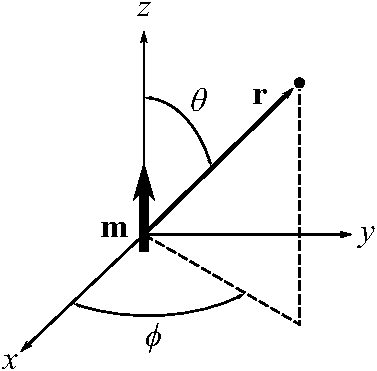
\includegraphics[width=4cm]{ch2/img/coord_pol_cart.pdf}
	\tdplotsetmaincoords{70}{110}
	\begin{tikzpicture}[auto,>=latex,tdplot_main_coords]
		\coordinate (origin) at (0,0,0);
		\tdplotsetrotatedcoords{-45}{-90}{0}
		\tdplotsetrotatedcoordsorigin{(origin)}
		%\riferimento
		% Axis
		\draw [->] (origin) -- (3,0,0) node[anchor=north east]{\scriptsize{$x$}}; \draw (origin) -- (-0.2,0,0);
		\draw [->] (origin) -- (0,2.5,0) node[anchor=west]{\scriptsize{$y$}}; \draw (origin) -- (0,-0.2,0);
		\draw [->] (origin) -- (0,0,2.5) node[anchor=south]{\scriptsize{$z$}}; \draw (origin) -- (0,0,-0.2);

		\draw[->,line width=2] (0,0,-0.1) -- node[left]{$\hat{\mathbf{m}}$} (0,0,1.5);
		\node [circle,draw,inner sep=1pt, fill=black] at (3,3,3) (rpoint) {};
		\draw [->] (origin) -- node[pos=0.8,above]{$\mathbf{r}$} (rpoint);
		\draw [dashed] (origin) -- (3,3,0) -- (3,3,3);
		\draw[tdplot_rotated_coords,<->] (2,0) arc (0:55:2) node[pos=0.5]{$\theta$};
		\draw [<->] (2,0,0) arc (0:45:2) node[pos=0.5,below]{$\phi$};
	\end{tikzpicture}
	\caption{From Polar coordinates to Cartesian coordinates}
	\label{fig:polar2cartesian}
\end{marginfigure}
\begin{marginfigure}
	\centering
	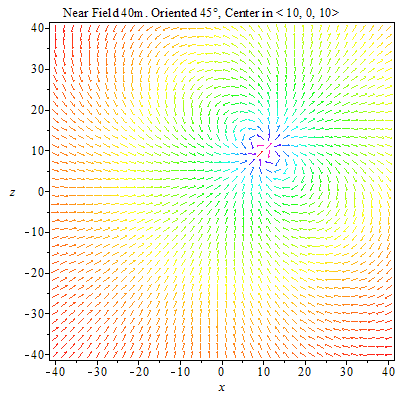
\includegraphics[width=5cm]{ch2/img/campo_casuale.png}
	\caption{Representation of a magnetic field with source: \newline $\postx = [10, 0, 10]^T$ \newline $\magdipole=[\ccos{\pi/4},0,\ssin{\pi/4}]^T$}
	\label{fig:dipolomagneticocasuale}
\end{marginfigure}
The last approximation is related to the nature of the receiver:
\begin{itemize}
\item the receiver act as an identifier of the constant quantity of the field, or the magnitude of the oscillating field
\item the distance of the receiver is always in a radius that allows us to not consider the effect of retarded potential: 
		\[\tau = \left. t - \dfrac{r}{c} \;\right|_{r\ll c}  \longrightarrow t \]
\end{itemize}

Under those considerations, and with MacLaurin first order transformation of $B_{\theta}$, the formulation of magnetic field real part takes the form:
\begin{equation}
\bfield = \dfrac{\magperm_0}{4 \pi r^3} \braces{ 2 m_0 \ccos{\theta} \vers{r} + m_0 \ssin{\theta} \vrtheta }
\label{eq:magneticfieldpolar}
\end{equation}

The projection of the field in cartesian coordinates is:
\begin{equation}
\bfield(\radiodist,\magdipole) = \dfrac{\magperm_0}{4 \pi r^5} \magfieldmatrix \magdipole
\end{equation}
A final generalization grants us the ability to write a general form of the field that has origin in position different from the origin:
\begin{equation}
\bfield(\hexastate - \postx,\magdipole)
\end{equation}
That is the form used for our simulations.

\section{Analytical signal analysis - A1--A \label{sec:a1asegnale}}

The ARTVA signal is a wild-life tag, specifically an \textbf{A--1A} signal. From the normative\cite{NormativaARVA}:
\begin{itemize}
\item A1A Signal:
	\begin{itemize}
	\item amplitude modulated signal
	\item digital information (keying)
	\item carrier frequency: \num{457}\si{\kilo\hertz}
	\item no auxiliary carrier
	\item frequency error shall not exceed $\pm$\num{80}\si{\hertz}
	\end{itemize}
\item carrier keying characteristics:
	\begin{itemize}
	\item on-time: \num{70}\si{\milli\second} minimum
	\item off-time: \num{400}\si{\milli\second} minimum
	\item period: \num{1000}\si{\milli\second} $\pm$ \num{300}\si{\milli\second}
	\end{itemize}
\item H--field peak at \num{10}\si{\meter}
	\begin{itemize}
	\item must be greater than \num{0.5}\si{\micro\ampere\per\meter}
	\item must be lower than \num{2.23}\si{\micro\ampere\per\meter}
	\end{itemize}
\end{itemize}

\begin{marginfigure}
	\centering
	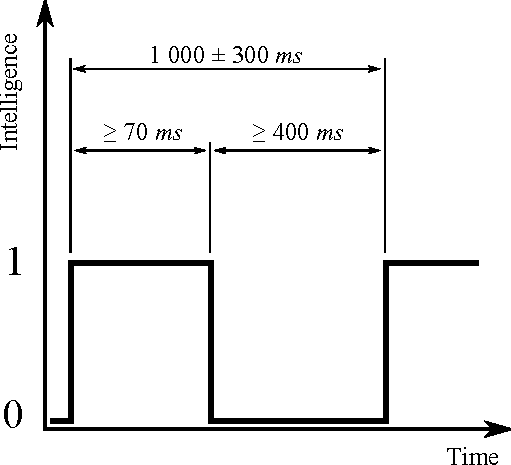
\includegraphics[width=5cm]{ch1/img/artva_signal.pdf}
	\caption{Intelligence signal of avalanche beacons}
	\label{fig:squarewaves}
\end{marginfigure}

The variable duty cycle is a challenge for the formulation of a searching algorithm, with a duty cycle ($\dutycycle$) that varies from a minimum of 5.4\% to a maximum of 42.9\%. The amplitude modulation, from a mathematical point of view is:
\begin{equation}
\jtx(t) = \braces{1+\mu \,\jint}\ccos{\omegaarva t}
\end{equation}
\begin{marginfigure}
	\centering
	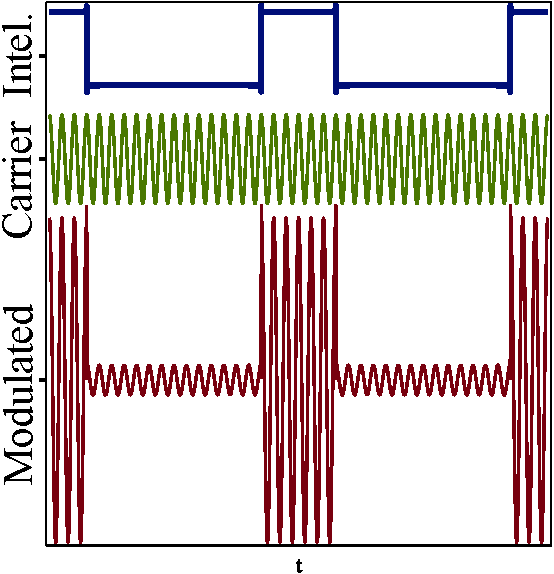
\includegraphics[width=5cm]{ch2/img/modulation_example.pdf}
	%\forceversofloat
	\caption{Example of a A--1A modulated signal}
	%\forceversofloat
\end{marginfigure}
There are 3 key elements:
\begin{itemize}
\item $\jint$ is the current of the intelligence signal, the representation of the square wave in figure \ref{fig:squarewaves}:
\begin{equation}
\jint(t) = A\dutycycle + \sum\limits_{n=1}^{\infty}\braces{\dfrac{2A}{n\pi}\ssin{n\pi \dutycycle} \ccos{\omegaint n t}}
\end{equation}
in which $A$ represents the signal amplitude and $\Delta$ is the duty cycle. 
\item the frequency of the carrier signal is ${f_0 = 2\pi\omegaarva}$, and it is \num{457}\si{\kilo\hertz}
\item $\mu$ is called modulation factor
\end{itemize}
From this current we are able to obtain the magnitude of dipole magnetic vector, using equation \ref{eq:dipolodacorrente}. Many of those parameter are device dependent and not known.

\section{Receiving antenna}

To receive such a long wavelenght for our appplication there is almost only one solution: use a ferrite core loop antenna, that is also the antenna used for transmission. In the next section, ferrite antenna is analyzed deeply, as a crucial part for the receiver. As we will see from the prototype, obtain a good receiver antenna is a very difficult task.

\subsection{Coils receiver}

\myparagraph{Single coil receiver}
\begin{marginfigure}
	\centering
	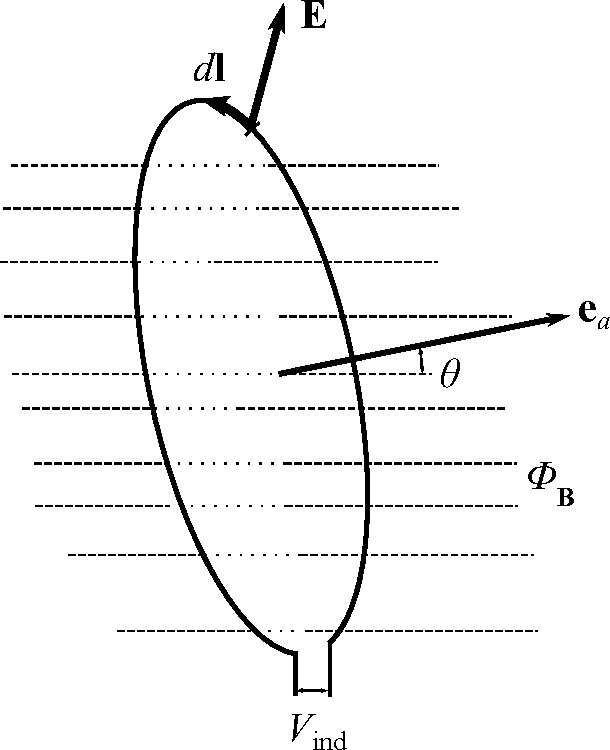
\includegraphics[width=5cm]{ch2/img/spira_singola.pdf}
	\caption{Single coil in field}
\end{marginfigure}
Under the hypothesys of an uniform EM field, using Maxwell's equations it is possible to derive potential difference induced in the coil:
\begin{equation}
\label{eq:tensioneindotta}
\vind = \oint\limits_{\diameter}\efield\cdot\mathbf{l} = -\dfrac{d\Phi_{\bfield}}{dt}
\end{equation}
where flux is:
\begin{equation}
\begin{array}{rcl}
\Phi_{\bfield} & = & \int\limits_{A_c} \bfield \cdot \hat{\mathbf{e}}_a dA \\
 & = & \magperm_0 H A \ccos{\theta}
\end{array}
\end{equation}
It is evident a cosine relation between field and axiis of the coil. The value of induced potential is maximum when the magnetic field $\hfield$ is orthogonal to the coil. $\theta$ is the angle between the field an the axis of the coil. Fusing two previous equations, we get:
\[
\vind = \magperm_0 A_c \dfrac{dH}{dt}
\]
that for our example:
\[
\vind = -j \omegaarva H A_c \magperm_0
\]
For conformity with the litterature, we express the magnetic field in terms of electric field\sidenote{It is known that: \newline $\magperm_{0} H = \dfrac{E}{\velocitaluce}$}:
\begin{equation}
\vind = \omegaarva \numerospire A_c \dfrac{E}{\velocitaluce}
\end{equation}

\myparagraph{Ferrite effect}
Inserting a ferrite bar brings to a deviation of the magnetic field flux. Fields lines are bended inside the ferrite because of its grater magnetic permeability
\begin{figure}
	\centering
	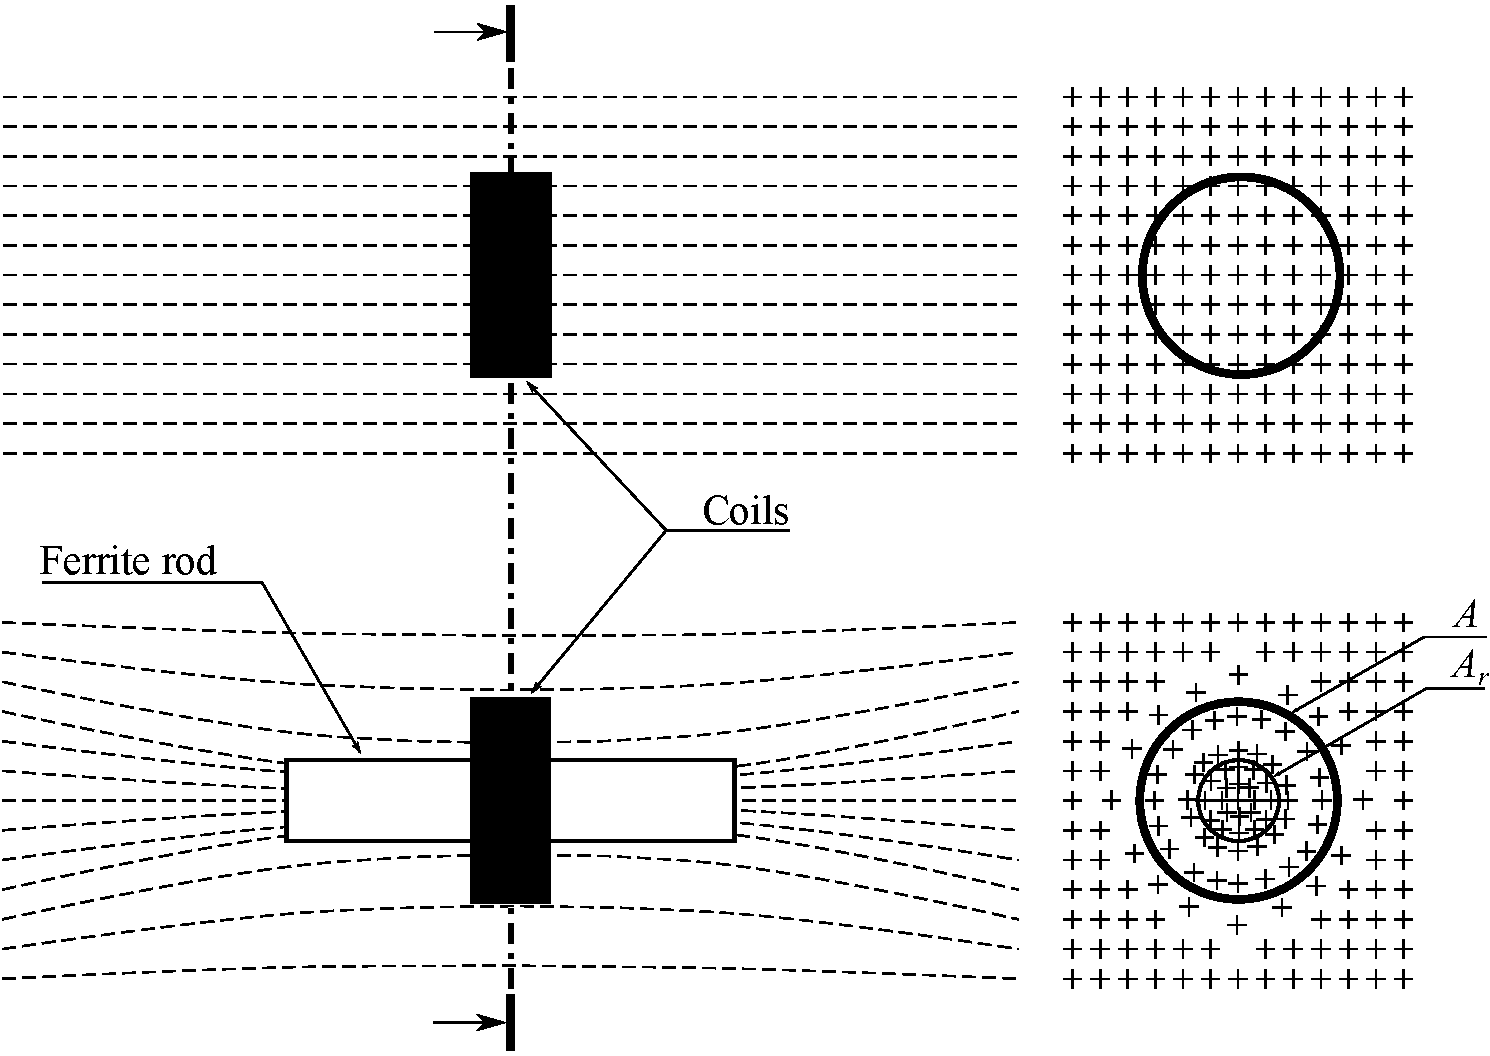
\includegraphics[width=11cm]{ch2/img/flux_lines.pdf}
	\label{fig:flussoferrite}
	\caption{Flux lines through coil and ferrite rod}
	\forceversofloat
\end{figure}
The total flux in section $A$ of figure \ref{fig:flussoferrite} is given by the flux that crosses area $A-A_r$ and flux that crosses area $A_r$:
\arraymath{
	\Phi_T & = & \Phi_{\bfield_1} + \Phi_{\bfield_2} \\
	\Phi_{\bfield_1} & = & \magperm_r A_r H \\
	\Phi_{\bfield_2} & = &\magperm_0 (A-A_r) H
}
and thus the total field is:
\begin{equation}
\Phi_T = H A_r \braces{ \magperm_r + \magperm_0 \braces{ \dfrac{A}{A_r} - 1} }
\end{equation}
bringing the previous equation in \ref{eq:tensioneindotta}, and simplifying with respect to constant parts of area, we get:
\begin{equation}
\vind = \omegaarva \numerospire \dfrac{E}{c} A_r \braces{\magperm_r + \braces{\dfrac{\diameter_c^2}{\diameter_r^2}-1}}
\end{equation}
In a real coil, we have a coil diameter that is equal to $\diameter_c = \diameter_c' + \diameter_\mathrm{wire}$, and it is usual to approximate $\diameter_c \approx \diameter_r$, and our antenna equation becomes:
\begin{equation}
\vind = \omegaarva \numerospire \dfrac{E}{c} A_r \magperm_r
\end{equation}
From which appears that the insertion of a ferrite rod in a coils inductance brings to an increase of induced tension proportional to the value of magnetic permeability of the ferrite itself. The identification of this value is not trivial and should be done experimentally. There are only some numerical approximation to the value of $\magperm_0$ related to the dimensions of ferrite bar, but it appears evidently a correlation between the ratio bar length/bar diameter. The greater this ratio, the greater the value of permeability\sidenote{We could give a trivial interpretation of this statement: the greater the length of the ferrite bar, the greater the number of flux lines that are bended into the bar; also the smaller the diameter, the grater the density of bended flux lines, thus the greater permeability value.}. 
\begin{equation}
\magperm_r \propto \dfrac{l_r}{\diameter_r}
\end{equation}

\myparagraph{Antenna effective height}
Effective height of antenna is defined as the ratio between the induced potential in the coils end the electric field intensity:
\begin{equation}
\altezzaeffettiva = \dfrac{\vind}{E}
\end{equation}
Applying previous equation to the definition of effective height:
\begin{equation}
\altezzaeffettiva = \dfrac{\omegaarva \numerospire A_r}{c} \braces{\magperm_r + \braces{\dfrac{\diameter_c^2}{\diameter_r^2}-1}}
\end{equation}

\subsection{Equivalent circuit and noise}
From a pure circuit point of view, ferrite antenna is seen as an an RLC circuit, in which we identify three passive components:
\begin{itemize}
\item $L\rightarrow\mathbf{Z}_L = j\omega L$: coil inductance
\item $R_p\rightarrow\mathbf{Z}_R = R_p$: wire resistance
\item $C\rightarrow\mathbf{Z}_C = (j\omega L)^{-1}$: parassite capacitance
\end{itemize}
The input voltage of the circuit is $\vind=\altezzaeffettiva E$
\begin{marginfigure}
	\centering
	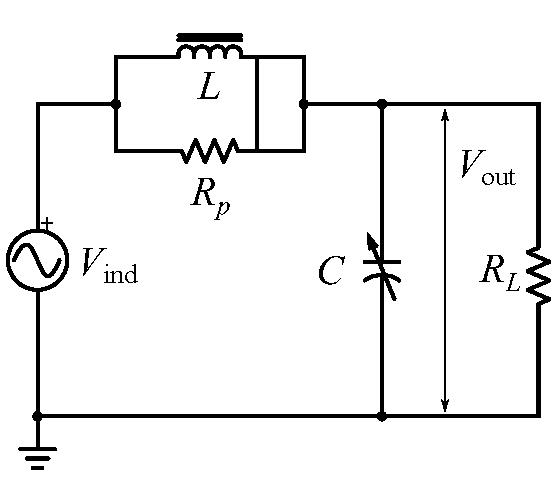
\includegraphics[width=5cm]{ch2/img/circuito_eq.pdf}
	\caption{Antenna equivalent circuit}
\end{marginfigure}

\myparagraph{Signal}
Starting from the definition of the equivalent circuit, with an external resistive load $R_L$ it is possible to derive a transfer function (full derivation in appendix at equation \ref{eq:transferfunc}):
\begin{equation}
\dfrac{V_{\mathrm{out}}}{\vind} = G(s) = \dfrac{\omega_{LC}}{Q_{\alpha}} \dfrac{s + Q_{\alpha} \omega_{LC}}{s^2 + \dfrac{\omega_{LC}}{Q_{\beta}} s + \omega_{LC}^2}
\end{equation}
\marginnote{\arraymath{
	\omega_{LC}^2 & = & \dfrac{1}{LC} \\
	Q_{\alpha} & = & \omega_{LC} R_P C \\
	Q_{\beta} & = & \omega_{LC} \dfrac{R_P R_L}{R_P + R_L} C
}}
if we obtain an $\omega_{LC} = \omegaarva$, we get resonance for an ARTVA incident signal: $s=j\omegaarva$:
\begin{equation}
G(j\omegaarva) = \left( -j Q_{\beta} \right) \left( 1 + \dfrac{j}{Q_{\alpha}} \right)
\end{equation} 
and then:
\begin{equation}
V_{\mathrm{out}} = \altezzaeffettiva \dfrac{Q_{\beta}}{Q_{\alpha}} E
\end{equation}

\myparagraph{Noise}
We could consider different sources of noise for our ferrite antenna:
\begin{itemize}
\item Boltzmann temperature noise
\item ferrite polarization noise
\item skin effect noise
\item auto-inductance noise
\end{itemize}

Even if some of those source are easily to model, some of them are not and require an experimental interpolation. For the Boltzmann withe noise:
\[
V_{n,B} = \sqrt{4 \boltzmann T \Delta f Q_{\beta} \mathbf{Z}_{L}}
\]
that is environment dependent. For the other sources, some more considerations must be driven. Skin effect and ferrite noise are proportional to the received field. 
Those two effects must be carefully taken into account and analyzed from experimental point of view. The first one is due to the distribution of the current in the section of the coil wire: current tends to accumulate in the skin layer of the wire, generating eddy currents that are sources of noise. To this effect, some special woven wire, like litz wire, should be used.
The second effect, ferrite noise, derives from the polarization of the magnetic crystal inside ferrite. To polarize the whole ferrite bar, some energy must be spent to move magnetic domain, and the movement of those domain generates a noise. This effect is strictly related to the quality of material and cannot be mitigated.
Auto-inductance noise is due to the current that is absorbed by the serial circuit of antenna and load. In a production of a prototype it is important that input of identification circuit has a very high impedance to reduce a generation of this current on antenna. Some high quality devices implement a secondary loop on the antenna that acts as a re-generator, that tries to null those parasitic currents effect.

It is straightforward now, that all those noise effect could be resumed in an unique interpolated expression $n \braces{\vind,T}$.

For simulation purpose it is possible to simulate this as Gaussian white noise as follows:
\begin{equation}
\sigma = N\braces{\mathbf{0}, V_{n,B}} + 10^{x} \abs{\vind} N\braces{\mathbf{0}, \Sigma}
\end{equation}
with $x$ a value that scales the proportional noise.
\section{Digital ARTVA prototype}
\begin{figure*}
	\centering
	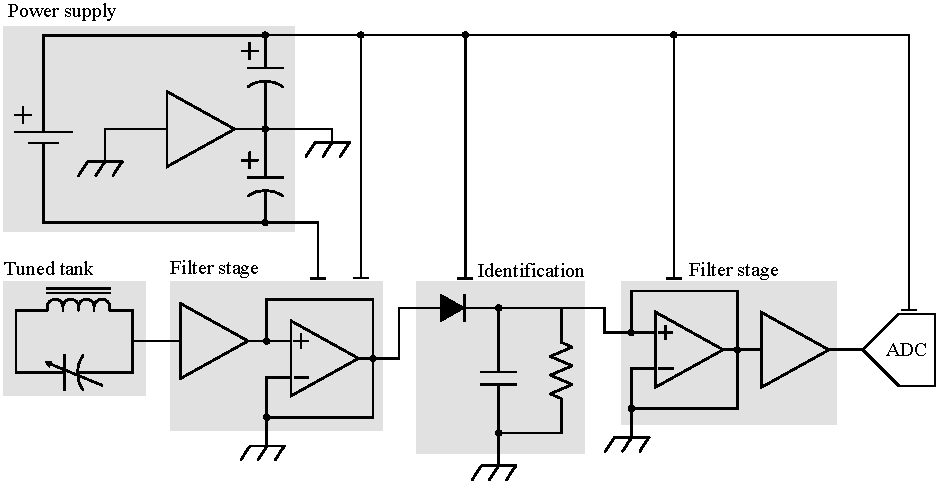
\includegraphics[scale=0.7]{ch2/img/block_circuit.pdf}
	\caption{Block diagram for the circuit}
	\label{fig:block_circuit}	
\end{figure*}
In the last section of this chapter, we use the knowledge collected to develop a prototype of an ARTVA receiver, in which there is not a transmission part. The receiver is the only fundamental module that we need for our drone, a transmitter will only be useless weight. 

In figure \ref{fig:block_circuit} there is the block outline of the device:
\begin{itemize}
\item the first block is the tuned tank, or tuned amplifier
\item the second block is the buffer and conditioner stage
\item the third block is the identification part
\item an amplification and a second buffer
\item digital component
\item dual supply stage
\end{itemize}
Through this section, each block will be discussed and explained. The design process has taken into account the tollerances for passive components\sidenote{Resistors: 5\%\newline Capacitors: 20\%}

\subsection{Tuned tank}
% \begin{figure}[b]
% 	\includegraphics[viewport=x y x y]{ch2/img/receiver3.pdf}
% 	\caption{}
% 	\label{fig:circuit}
% 	%\forceversofloat
% \end{figure}
\begin{figure}[h]
	\centering
	\includegraphics*[viewport=3 3 240 457,scale=0.4]{ch2/img/receiver3.pdf}
	\caption{Tuned tank portion of circuit}
	\label{fig:tunedtank}
	%\forceversofloat
\end{figure}

The tuned tank is composed by a ferrite antenna, with a rod of \num{10}\si{\centi\meter} per \diameter \num{1}\si{\centi\meter}. The wire of the coil is a \num{30} AWG enameled copper wire, with a final parasite resistance of \num{22}\si{\ohm}. The coil as \num{70} windings. For more informations about this tuned circuit, check previous section.

\subsection{Buffer and filter}
\begin{figure*}[h]
	\centering
	\includegraphics*[viewport=170 3 1250 380,scale=0.4]{ch2/img/receiver3.pdf}
	\caption{First filter stage}
	\label{fig:filter1}
	%\forceversofloat
\end{figure*}

This block is composed by a first stage that acts as a separation between the tuned tank and the filter, thus is also called voltage follower. To limit the number of components on the board this stage is obtained with an operational amplifier. To grant a longer receiving range, an high--gain selective active filter is in cascade to the buffer before the identification. It is important to select an operational amplifier with an high bandwidth--gain--product to grant the gain at \num{457}\si{\kilo\hertz}, at which the filter is centered. Also, this stage depends to the dual \num{\pm 5}\si{\volt} supply stage. 
\begin{marginfigure}
	\centering
	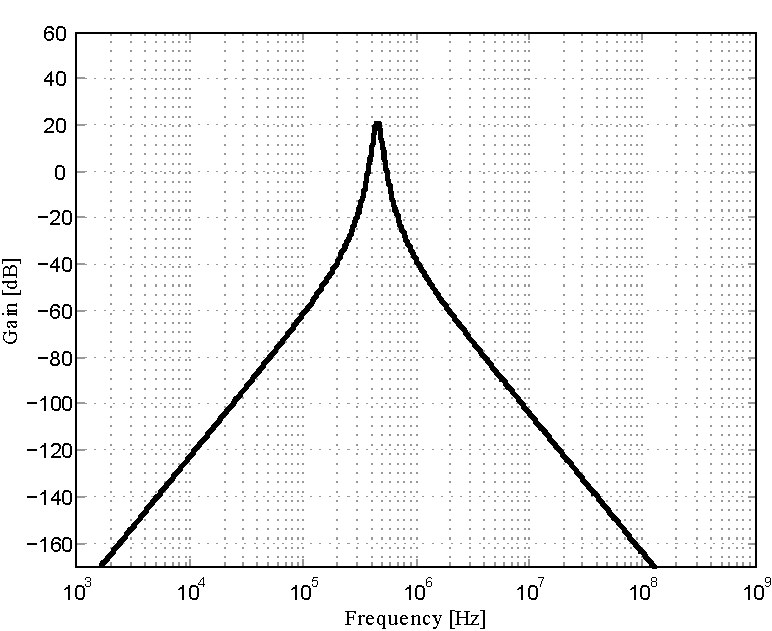
\includegraphics[width=5cm]{ch2/img/filter1.pdf}
	\caption{Filter magnitude characteristic}
\end{marginfigure}

The op--amp chosen is \texttt{LF347N}, even if a faster amplifier may be selected, it is advised to stay below the \num{60}\si{\mega\hertz} BW, to avoid auto--resonance effects.

\subsection{Identification}
\begin{figure}[h]
	\centering
	\includegraphics*[viewport=1251 3 1580 595,scale=0.4]{ch2/img/receiver3.pdf}
	\caption{Identification stage}
	\label{fig:identifier}
	%\forceversofloat
\end{figure}
\begin{marginfigure}
	\centering
	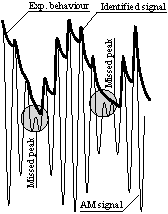
\includegraphics[width=4.5cm]{ch2/img/identificatore.pdf}
	\caption{Logical function of an identifier}
	\label{fig:identifier_log}
\end{marginfigure}
The central part of the circuit is an identification circuit, obtained with the monolithic classical IC \texttt{TA7641}\sidenote{A.k.a.: \texttt{MK484} or \texttt{ZN414}},  that acts as a one chip radio solution in AM. All receiver is derived from the modification of the basic circuit provided in schematics of this IC, extended with filtering and buffers, and the removal of the auto gain control resistance in the output feedback. Also, transistor amplification stage is removed. The output of this circuitry is in \numrange{40}{60}\si{\milli\volt}, with a very low current required. The input pin has a good impedance 

To better understand the use of this stage, look at figure \ref{fig:identifier_log}, in which an extremely simplified version of the IC is represented with common components. The IC straightens the received signal and identifies the envelope of the modulated intelligence with a low pass filter that has a dynamic not too slow, to not loose some of the higher frequencies information modulated (also called missed peak). IC implements this function with an high quality envelope detector.
\begin{figure*}[h]
	\centering
	\includegraphics*[viewport=1443 3 2320 350,scale=0.4]{ch2/img/receiver3.pdf}
	\caption{Low pass filter and amplification stage}
	\label{fig:filter2}
	\forceversofloat
\end{figure*}

\subsection{Amplifier}

The identified signal is, again, amplified and filtered, to a lower frequency, to grant the isolation of the square wave, with respect to the residual carrier and other source of interference. A \num{10}\si{\decibel} gain filter, with 2 stages was implemented. After the filter, another buffer connects analog circuitry with digital micro--controller.
\begin{marginfigure}
	\centering
	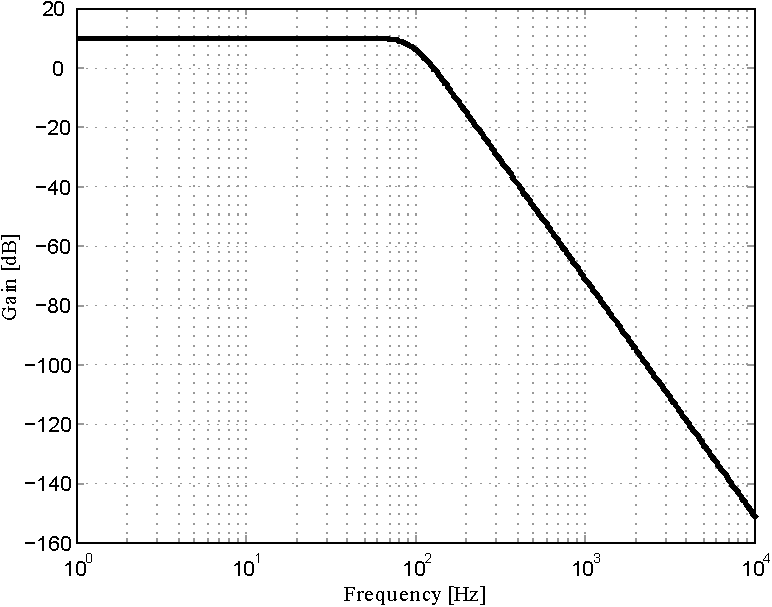
\includegraphics[width=5cm]{ch2/img/filter2.pdf}
	\caption{Filter magnitude characteristic}
\end{marginfigure}

\subsection{Digital stage}
\begin{figure}[h]
	\centering
	\includegraphics*[viewport=2320 3 2650 350,scale=0.4]{ch2/img/receiver3.pdf}
	\caption{Digital stage}
	\label{fig:adc}
	%\forceversofloat
\end{figure}
One last stage is he ADC and the UART interface on the micro--controller. Using an \texttt{MSP430} it is easy to develop in \texttt{C} the routines necessary to perform the task. To reduce the power consumption, ADC sampling is performed with ALU in power saving mode. Once the sampling task is completed, an interrupt brings up the ALU that set up the variables too be sent over serial interface UART (or SPI or I2C).

\subsection{Dual supply}
The supply is obtained through the use of a virtual ground and a symmetrical classical regulation circuit. This scheme is sometimes called rail splitter, and it is necessary for the first regulation stage, to avoid op--amps saturation.
\begin{figure}[h]
	\centering
	\includegraphics*[viewport=3 450 580 750,scale=0.4]{ch2/img/receiver3.pdf}
	\caption{Example of a sampling result}
	\label{fig:sampling_res}
	\forceversofloat
\end{figure}

\subsection{Tri--axes ARTVA}
In figure \ref{fig:sampling_res} there is an example of sampling from the real prototype, using MATLAB serial reading capabilities. A complete prototype uses three equal antenna--filter--identification--amplifier stage, with orthogonal antennas, and one single ADC micro--controller and power supply.
\begin{figure}[h]
	\centering
	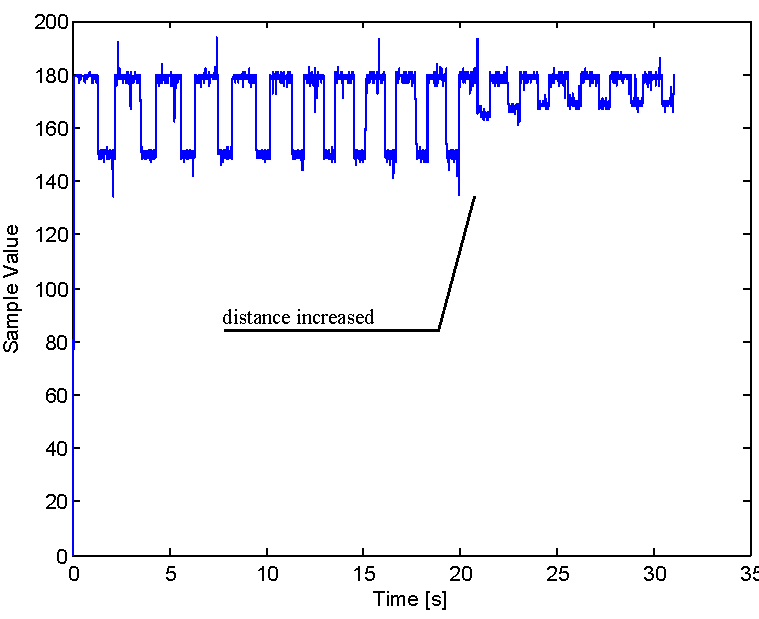
\includegraphics[scale=0.65]{ch2/img/sampling_result.pdf}
	\caption{Complete circuit}
	\label{fig:completecirc}
	%\forceversofloat
\end{figure}
\begin{figure}[p]
	\centering
	\includegraphics[scale=0.25,angle=90]{ch2/img/receiver3.pdf}
	\caption{Complete circuit}
	\label{fig:completecirc}
	\forceversofloat
\end{figure}

%\FloatBarrier
\clearpage
%%%%%%%%%% Appendix %%%%%%%%%%%%%%%%%%%%%%%%%%%%%%%%%%%%
% Appendix of chapter 2

\section{Appendix}

\subsection{Polar coordinates}

Maps:
\begin{equation} \left\{ \begin{array}{rcl} x & = & r \sin(\theta) \cos(\phi) \\ y & = & r \sin(\theta) \sin(\phi) \\ z & = & r \cos(\theta) \end{array}\right. \rightarrow \left\{ \begin{array}{rcl} r & = & \sqrt{x^2+y^2+z^2} \\ \theta & = & \arctan\left(\dfrac{z}{\sqrt{x^2+y^2}}\right) \\ \phi & = & \arctan\left( \dfrac{x}{y} \right) \end{array} \right. \end{equation}

Versors in Cartesian coordinates:
\begin{equation} \left[ \begin{array}{ccc} \vrr & \vrtheta & \vrphi \end{array}\right] = \dfrac{1}{\sqrt{x^2+y^2+z^2}} \left[ \begin{array}{ccc} x & \dfrac{xz}{\sqrt{x^2+y^2}} & -\dfrac{y}{\sqrt{x^2+y^2}} \\ y & -\dfrac{yz}{\sqrt{x^2+y^2}} & \dfrac{x}{\sqrt{x^2+y^2}} \\ z & -\dfrac{x^2+y^2}{\sqrt{x^2+y^2}} & 0 \end{array} \right] \end{equation}

\subsection{Evidences}

\myparagraph{EM field dynamic potential}
The following equations are the proof for \ref{eq:potvecmaxwell}
\begin{equation}
\begin{array}{rcl}
\nabla \cdot \left(  - \nabla \scpot - \partialtarg{\afield} \right) & = & \dfrac{\chargedens}{\dielettrico_0} \\
\nabla^2 \scpot + \partialt{\nabla \cdot \afield} & = & -\dfrac{\chargedens}{\dielettrico_0} \\
 & & \\
\magperm_0 \left( \currdens + \dielettrico_0 \partialt\left(- \nabla \scpot - \partialtarg{\afield}\right) \right) & = & \nabla \times \left( \nabla \times \afield \right) \\
\magperm_0 \currdens - \magperm_0 \dielettrico_0 \dfrac{\partial^2 \afield}{\partial t^2} - \magperm_0 \dielettrico_0 \nabla \dfrac{\partial \scpot}{\partial t} & = & \nabla \left( \nabla \cdot \afield \right) - \nabla^2 \afield \\
\nabla^2 \afield - \dfrac{1}{c^2} \dfrac{\partial^2 \afield}{\partial t^2} - \nabla \left( \nabla \cdot \afield + \dfrac{1}{c^2} \dfrac{\partial \scpot}{\partial t} \right) & = & - \magperm_0 \currdens
\end{array}
\label{eq:evidence1}
\end{equation}

In the following equation invariance with respect to recalibration map is showed:
\begin{equation}
\label{eq:prooftransformationmap}
\begin{array}{rcl}
\nabla \times \afield' & = & \nabla(\afield + \nabla \lorentz) \\
 & = & \nabla \times \afield + \nabla \times \nabla \lorentz \\
 & = & \nabla \times \afield \\
 & = & \bfield \\
 & & \\
- \nabla\scpot' - \partialtarg{\afield'} & = & -\nabla \left( \scpot - \partialtarg{\lorentz} \right) - \partialt\left( \afield + \nabla \lorentz \right) \\
 & = & -\nabla \scpot + \nabla \partialt \lorentz - \partialtarg{\afield} - \partialt\nabla\lorentz \\
 & = & -\nabla \scpot - \partialtarg{\afield} \\
 & = & \efield
\end{array}
\end{equation}

\myparagraph{Magnetic dipole radiation}
To evaluate the integral \ref{eq:integraledacalc}  we should consider some simplifications.

$r' \ll r$: for an ideal dipole, coils radius shall be really with respect to radio vector:
\[
\begin{array}{rcl}
\kappa & = & \sqrt{(\radiodist - \radiodist') \cdot (\radiodist - \radiodist')} = \\
 & = & \sqrt{\radiodist \cdot \radiodist + \radiodist' \cdot \radiodist' - 2\; \radiodist \cdot \radiodist'} \\
 & = & \sqrt{r^2 + r'^2 - 2\,r\,r'\,sin(\theta)cos(\varphi')} \\
 & = & r\;\sqrt{1 + \dfrac{r'^2}{r^2} - 2\,\dfrac{r'}{r}\,sin(\theta)cos(\varphi')}
\end{array}
\]
the simplification is performed by the use of Taylor expansions, under the hypothesis of $r'^2/r^2 \approx 0$:
\arraymath{
\kappa & = & \mathrm{Taylor}_2\left[ r\;\sqrt{1 - 2\,\dfrac{r'}{r}\,sin(\theta)cos(\varphi')} \right]_{\dfrac{r'}{r} \rightarrow 0} \\
 & \approx & r\left( 1 - \dfrac{r'}{r}\,sin(\theta)cos(\varphi') \right)
}
imposing the inverse:
\arraymath{
\dfrac{1}{\kappa} & = & \dfrac{1}{r}\left( 1 - \dfrac{r'}{r}\,sin(\theta)cos(\varphi') \right)^{-1} \\
 & = & \mathrm{Taylor}_2\left[ \dfrac{1}{r}\left( 1 - \dfrac{r'}{r}\,sin(\theta)cos(\varphi') \right)^{-1} \right]_{\dfrac{r'}{r} \rightarrow 0} \\
 & \approx & \dfrac{1}{r}\left( 1 - \dfrac{r'}{r}\,sin(\theta)cos(\varphi') \right)
}

$r' \ll \lambda = 2\pi\velocitaluce/\omegaarva$: this observation permits us to simplify the cosine in the argument of the integral, with $\tau$ as defined in \ref{eq:campidef1}:
\marginnote{$\cos(\gamma + \beta) = \cos\gamma\cos\beta - \sin\gamma\sin\beta$\\for $\gamma\rightarrow0$ we get $\ssin{\gamma} \approx \omegaarva\tau$ and $\ccos{\gamma} \approx 1$}
\arraymath{
\ccos{\omegaarva \left( t - \dfrac{\kappa}{\velocitaluce}\right)} & \approx & \ccos{\omegaarva\tau} + \dfrac{\omegaarva r'}{\velocitaluce} \ssin{\theta} \ccos{\varphi'} \\
 & = & \ccos{\omegaarva\tau}\ccos{\dfrac{\omegaarva r'}{\velocitaluce} \ssin{\theta} \ccos{\varphi'}} - \\
 &   & + \ssin{\omegaarva\tau} \ssin{\dfrac{\omegaarva r'}{\velocitaluce} \ssin{\theta} \ccos{\varphi'}} \\
 & \approx & \ccos{\omegaarva\tau} - \\ & & + \ssin{\omegaarva\tau} \ssin{\dfrac{\omegaarva r'}{\velocitaluce} \ssin{\theta} \ccos{\varphi'}}
}

The union of the two simplifications give us as integral argument:
\[\begin{array}{l}
\dfrac{1}{r}\braces{1+\dfrac{r' \ccos{\theta} \ssin{\varphi'}}{r}} \cdot \\
\cdot \braces{\ccos{\omegaarva\tau} - \dfrac{\omegaarva r' \ssin{\theta} \ccos{\varphi'}\ssin{\omegaarva\tau}}{\velocitaluce}}
\end{array}\]
expanding and considering $\xi = \ssin{\theta}\ccos{\varphi'}$ we obtain:
\[
\dfrac{1}{r} \braces{ \dfrac{\omegaarva\ssin{\omegaarva\tau}\xi r'}{c} + \ccos{\omegaarva\tau} - \dfrac{\omegaarva\ssin{\omegaarva\tau}\xi r'^2}{cr} + \dfrac{\ccos{\omegaarva\tau}\xi r'}{r} }
\]
where the term $\frac{r'^2}{cr} = \frac{r'}{r}\;\frac{\omegaarva}{2\pi}\;\frac{r'}{\lambda} \approx 0$ as we have already stated:
\[
\dfrac{1}{r} \braces{ \ccos{\omegaarva\tau} -\braces{\dfrac{\omegaarva}{c}\ssin{\omegaarva\tau} - \dfrac{1}{r}\ccos{\omegaarva\tau}}r'\xi}
\]
extracting only the parts that are function of integration variable $\varphi'$:
\arraymath{
a_1 & = & \dfrac{1}{r} \ccos{\omegaarva\tau} \\
a_2 & = & \dfrac{1}{r} \braces{\dfrac{\omegaarva}{c}\ssin{\omegaarva\tau} - \dfrac{1}{r}\ccos{\omegaarva\tau}}r'\ssin{\theta}
}
The final integral is in the form:
\[
\afield(\radiodist,t) = \dfrac{\magperm_0 J_0 r'}{4\pi r} \int\limits_{0}^{2\pi}a_1 \ccos{\varphi'} - a_2 \cos^2\braces{\varphi'} d\varphi' \hat{\phi}
\]
and thus solved:
\marginnote{$\begin{array}{l} \int\limits_0^{2\pi}\ccos{\varphi'}d\varphi' = 0 \\ \int\limits_0^{2\pi}\cos^2\braces{\varphi'}d\varphi' = \pi \end{array}$}
\arraymath{
\afield(\radiodist,t) & = & -\dfrac{\magperm_0 J_0 r'}{4\pi} \pi a_2 \\
 & = & \dfrac{\magperm_0 J_0 r'^2 \pi}{4\pi r} \braces{\dfrac{1}{r}\ccos{\omegaarva\tau} - \dfrac{\omegaarva}{c}\ssin{\omegaarva\tau}}
}
Applying the substitution $m_0 = \pi r'^2 J_0$ we found the solution reported in equation \ref{eq:soluzioneint}.

\myparagraph{Complex version of magnetic field}
Here the proof of complex magnetic field equations:
\[
\begin{array}{rcl}
B_r & = & \dfrac{1}{2} \dfrac{\magperm_0 m_0}{\pi} \ccos{\theta} \braces{\dfrac{1}{r^3}\ccos{\omegaarva \tau} - \dfrac{\kappa}{r^2} \ssin{\omegaarva \tau}} \\
 & = & \dfrac{1}{2} \dfrac{\magperm_0 m_0}{\pi} \ccos{\theta} \kappa^3 \braces{ \dfrac{1}{r^3 \kappa^3} \ccos{\omegaarva\tau} - \dfrac{1}{r^2 \kappa^2} \ssin{\omegaarva\tau} } \\
 & = & \dfrac{1}{2} \dfrac{\magperm_0 m_0}{\pi} \ccos{\theta} \kappa^3 \braces{ \dfrac{1}{r^3 \kappa^3} + \dfrac{j}{r^2 \kappa^2}} e^{j\omegaarva \tau} \\
 & = & \dfrac{1}{2} \dfrac{\magperm_0 m_0}{\pi} \ccos{\theta} \kappa^3 \braces{ \dfrac{j}{r^2 \kappa^2} + \dfrac{1}{r^3 \kappa^3}} e^{j\omegaarva \tau} \\
 & = & -\dfrac{1}{2} j \dfrac{\magperm_0 m_0}{\pi} \kappa^3 \ccos{\theta} \braces{\dfrac{1}{j^2 r^2 \kappa^2} + \dfrac{1}{j^3 r^3 \kappa^3}} e^{j\omegaarva \tau}
\end{array}
\]

\[
\begin{array}{rcl}
B_{\theta} & = & \dfrac{1}{4} \dfrac{\magperm_0 m_0}{\pi r^3 c^2} \ssin{\theta} \braces{\braces{\velocitaluce^2 - \omegaarva^2 r^2}\ccos{\omegaarva \tau} - \omegaarva r \velocitaluce \ssin{\omegaarva \tau}} \\
 & = & \dfrac{1}{4} \dfrac{\magperm_0 m_0}{\pi} \ssin{\theta} \braces{ \braces{\dfrac{1}{r^3}-\dfrac{\omegaarva^2}{c^2 r}}\ccos{\omegaarva \tau} - \dfrac{\omegaarva}{r^2 c} \ssin{\omegaarva \tau}} \\
 & = & \dfrac{1}{4} \dfrac{\magperm_0 m_0}{\pi} \ssin{\theta} \braces{ \braces{\dfrac{1}{r^3}-\dfrac{\kappa^2}{r}}\ccos{\omegaarva \tau} - \dfrac{\kappa}{r^2} \ssin{\omegaarva \tau}} \\
 & = & \dfrac{1}{4} \dfrac{\magperm_0 m_0}{\pi} \ssin{\theta} \kappa^3 \braces{ \braces{\dfrac{1}{r^3 \kappa^3}-\dfrac{1}{r \kappa}}\ccos{\omegaarva \tau} - \dfrac{1}{r^2 \kappa^2} \ssin{\omegaarva \tau}} \\
 & = & \dfrac{1}{4} \dfrac{\magperm_0 m_0}{\pi} \ssin{\theta} \kappa^3 \braces{ \braces{\dfrac{1}{r^3 \kappa^3}-\dfrac{1}{r \kappa}} + \dfrac{j}{r^2 \kappa^2}} e^{j\omegaarva \tau} \\
 & = & \dfrac{1}{4} \dfrac{\magperm_0 m_0}{\pi} \ssin{\theta} \kappa^3 \braces{-\dfrac{1}{r \kappa} + \dfrac{j}{r^2 \kappa^2} + \dfrac{1}{r^3 \kappa^3}} e^{j\omegaarva \tau} \\
 & = & -\dfrac{1}{4} j \dfrac{\magperm_0 m_0}{\pi} \kappa^3 \ssin{\theta} \braces{\dfrac{1}{j r \kappa} + \dfrac{1}{j^2 r^2 \kappa^2} + \dfrac{1}{j^3 r^3 \kappa^3}} e^{j\omegaarva \tau}
\end{array}
\]

\myparagraph{The field in cartesian coordinates}
From the figure \ref{fig:polar2cartesian} we derive the following relations:
\arraymath{
\vers{r} & = & \dfrac{\radiodist}{\abs{\radiodist}} \\
\vrtheta & = & \dfrac{ (\magdipole \times \radiodist) \times \radiodist }{ \abs{ (\magdipole \times \radiodist) \times \radiodist } } 
}
and the magnetic dipole vector is the projection on the two versors:
\arraymath{
\magdipole \cdot \vers{r} & = & m_0 \ccos{\theta}\\
\magdipole \cdot \vrtheta & = & -m_0 \ssin{\theta}
}
thus equation \ref{eq:magneticfieldpolar} becomes:
\arraymath{
\bfield & = & \dfrac{\magperm_0}{4 \pi r^3} \braces{ 2 m_0 \ccos{\theta} \vers{r} + m_0 \ssin{\theta} \vrtheta } \\
 & = & \dfrac{\magperm_0}{4 \pi r^3}\braces{2\braces{\magdipole \cdot \vers{r}} \vers{r} - \braces{\magdipole \cdot \vrtheta} \vartheta} \\ 
 & = & \dfrac{\magperm_0}{4 \pi r^3}\braces{3\braces{\magdipole \cdot \vers{r}} \vers{r} - \braces{\magdipole \cdot \vers{r}} \vers{r} - \braces{\magdipole \cdot \vrtheta} \vartheta} \\ 
 & = & \dfrac{\magperm_0}{4 \pi r^3}\braces{3\braces{\magdipole \cdot \vers{r}} \vers{r} - \magdipole}
}
putting the last equation in an analytical math engine, we derive this compact version, using as notation $\radiodist = [x,\,y,\,z]^T$:
\begin{equation}
\bfield = \dfrac{\magperm_0}{4 \pi r^5} \magfieldmatrix \magdipole
\end{equation}

\subsection{Antenna transfer function}
It is easy to derive transfer function, if we consider the system as a voltage divider:
\begin{equation}\label{eq:transferfunc}
\begin{array}{ccl}
\dfrac{V_{\mathrm{out}}}{\vind} & = & \dfrac{\left(R_L \parallel C s \right)}{\left(R_L \parallel C s \right) + \left(R_P \parallel L s \right)} \\
& = & \dfrac{\dfrac{1}{\dfrac{1}{R_L} + Cs}}{\dfrac{1}{\dfrac{1}{R_L} + Cs} + \dfrac{1}{\dfrac{1}{R_L} + \dfrac{1}{L s}}} \\
& = & \dfrac{ \dfrac{1}{R_p}+\dfrac{1}{Ls} }{ \dfrac{1}{R_L} + Cs + \dfrac{1}{R_P} + \dfrac{1}{Ls} } \\
& = & \dfrac{1}{R_P C} \dfrac{s + \dfrac{R_P}{L}}{s^2 + \dfrac{1}{C \dfrac{R_P R_L}{R_P + R_L}}s + \dfrac{1}{LC}} 
\end{array}
\end{equation}




\backmatter
		\listofsymbolspages
		%\showthe\parskip
		\setlength{\parskip}{5pt}
		\bibliographyinsert
		\setlength{\parskip}{0pt}
		%\index ?? we will see

\end{document}